% \documentclass[9pt,aspectratio=169]{beamer}
\documentclass[9pt,xcolor={dvipsnames}]{beamer}
% packages
\usepackage{amsmath}
\usepackage{amsthm}
\usepackage{amssymb}
\usepackage{mdframed}
\usepackage{subcaption}
\usepackage{cite}
\usepackage[dvipsnames]{xcolor}
\usepackage{tikz}
\usepackage{float}
\usepackage{tikz-cd}
\usepackage{dashbox}
\usepackage[normalem]{ulem}
\usepackage{bbm}
\usepackage{fancyhdr}
\newcommand\graphnode[1]{\begin{tabular}{@{}c@{}}#1\end{tabular}}
\usepackage{pgfplots}
\pgfplotsset{compat=newest}
\usepgfplotslibrary{fillbetween}
\usepackage{environ}
\makeatletter
\newsavebox{\measure@tikzpicture}
\NewEnviron{scaletikzpicturetowidth}[1]{%
  \def\tikz@width{#1}%
  \def\tikzscale{1}\begin{lrbox}{\measure@tikzpicture}%
  \BODY
  \end{lrbox}%
  \pgfmathparse{#1/\wd\measure@tikzpicture}%
  \edef\tikzscale{\pgfmathresult}%
  \BODY
}
\makeatother
\usetikzlibrary{hobby}
\usetikzlibrary{shapes.misc}
\usepackage[backref=page]{hyperref}
\hypersetup{
    breaklinks=true,
    colorlinks=true,
    urlcolor=urlcolor,
    linkcolor=linkcolor,
    citecolor=citecolor,
    }

\usepackage{booktabs}
\usepackage{enumitem}
\setlist[itemize]{noitemsep}
\setlist[enumerate]{noitemsep}


% commands
% symbols =======================
% mathbb
\newcommand{\NN}{\mathbb{N}}
\newcommand{\ZZ}{\mathbb{Z}}
\newcommand{\QQ}{\mathbb{Q}}
\newcommand{\XX}{\mathbb{X}}
\newcommand{\RR}{\mathbb{R}}
\renewcommand{\SS}{\mathbb{S}}
\newcommand{\CC}{\mathbb{C}}
\newcommand{\KK}{\mathbb{K}}
\newcommand{\HH}{\mathbb{H}}
\newcommand{\EE}{\mathbb{E}}
\newcommand{\PP}{\mathbb{P}}
\newcommand{\WW}{\mathbb{W}}
% mathcal
\newcommand{\Aa}{\mathcal{A}}
\newcommand{\Bb}{\mathcal{B}}
\newcommand{\Rr}{\mathcal{R}}
\newcommand{\Cc}{\mathcal{C}}
\newcommand{\Dd}{\mathcal{D}}
\newcommand{\Ee}{\mathcal{E}}
\newcommand{\Hh}{\mathcal{H}}
\newcommand{\Ff}{\mathcal{F}}
\newcommand{\Gg}{\mathcal{G}}
\newcommand{\Ii}{\mathcal{I}}
\newcommand{\Ll}{\mathcal{L}}
\newcommand{\Nn}{\mathcal{N}}
\newcommand{\Mm}{\mathcal{M}}
\newcommand{\Oo}{\mathcal{O}}
\newcommand{\Pp}{\mathcal{P}}
\newcommand{\Qq}{\mathcal{Q}}
\newcommand{\Ss}{\mathcal{S}}
\newcommand{\Tt}{\mathcal{T}}
\newcommand{\Vv}{\mathcal{V}}
\newcommand{\Ww}{\mathcal{W}}
\newcommand{\Xx}{\mathcal{X}}
\newcommand{\Yy}{\mathcal{Y}}
\newcommand{\Zz}{\mathcal{Z}}
% letters
\newcommand{\al}{\alpha}
\newcommand{\be}{\beta}
\newcommand{\ga}{\gamma}
\newcommand{\de}{\delta}
\newcommand{\eps}{\varepsilon}
\renewcommand{\th}{\theta}
\newcommand{\la}{\lambda}
\newcommand{\si}{\sigma}
\newcommand{\om}{\omega}
\newcommand{\Ga}{\Gamma}
\newcommand{\De}{\Delta}
\newcommand{\La}{\Lambda}
\newcommand{\Si}{\Sigma}
\newcommand{\Om}{\Omega}
\renewcommand{\phi}{\varphi}
\renewcommand{\epsilon}{\varepsilon}

% operators ==========
\renewcommand{\ker}{\operatorname{Ker}}
\DeclareMathOperator*{\rk}{rk}
\DeclareMathOperator*{\diag}{diag}
\DeclareMathOperator*{\card}{card}
\DeclareMathOperator*{\sgn}{sgn}
\DeclareMathOperator*{\argmax}{arg\,max}
\DeclareMathOperator*{\argmin}{arg\,min}
\newcommand{\scal}[2]{\left\langle #1,\, #2 \right\rangle}
\newcommand{\enscond}[2]{\left\lbrace #1,\quad #2 \right\rbrace}
\newcommand{\pd}[2]{ \frac{ \partial #1}{\partial #2} }
\newcommand{\umin}[1]{\underset{#1}{\min}\;}
\newcommand{\umax}[1]{\underset{#1}{\max}\;}
\newcommand{\uargmin}[1]{\underset{#1}{\argmin}\;}
\newcommand{\uargmax}[1]{\underset{#1}{\argmax}\;}
\newcommand{\norm}[1]{\left\|#1\right\|}
\newcommand{\abs}[1]{\left|#1\right|}
\newcommand{\pa}[1]{\left(#1\right)}
\newcommand{\bra}[1]{\left[#1\right]}
\newcommand{\cro}[1]{\left\{#1\right\}}
\newcommand{\set}[1]{\left\{#1\right\}}
\DeclareMathOperator{\KL}{KL}
\newcommand{\KLdiv}[2]{\KL\pa{#1 | #2}}
\newcommand{\KLproj}{\text{Proj}^{\tiny\KL}}
\newcommand{\choice}[1]{ \left\{ \begin{array}{l} #1 \end{array} \right. }
\def\ones{\mathbbm{1}}
\def\id{\operatorname{id}}
\def\anti{\operatorname{anti-id}}
\newcommand{\graph}{\mathrm{gph}}
% text
\newcommand{\qandq}{\quad\text{and}\quad}
\newcommand{\qwhereq}{\quad\text{where}\quad}
\newcommand{\qifq}{\quad\text{if}\quad}
\newcommand{\qarrq}{\quad\Longrightarrow\quad}
\newcommand{\as}{\text{as }}
\newcommand{\qas}{\quad\text{as }}
\newcommand{\where}{\text{where }}
\newcommand{\tmin}{\text{min}}
\newcommand{\tmax}{\text{max}}

% mathrm
\newcommand{\dd}{\,\mathrm d}

% Mark sections of captions for referring to divisions of figures
\newcommand{\figleft}{{(Left)}}
\newcommand{\figcenter}{{(Center)}}
\newcommand{\figright}{{(Right)}}
\newcommand{\figtop}{{(Top)}}
\newcommand{\figbottom}{{(Bottom)}}
\newcommand{\captiona}{{(a)}}
\newcommand{\captionb}{{(b)}}
\newcommand{\captionc}{{(c)}}
\newcommand{\captiond}{{(d)}}

\newcommand{\defeq}{\triangleq}

\usepackage[capitalize]{cleveref}
\crefname{section}{Sec.}{Sec.}
\Crefname{section}{Section}{Sections}
\Crefname{table}{Table}{Tables}
\crefname{table}{Tab.}{Tabs.}
\crefname{equation}{}{}
\Crefname{equation}{Eq.}{}

\definecolor{tabblue}{rgb}{0.12156862745098039, 0.4666666666666667, 0.7058823529411765}
\definecolor{tabblue}{rgb}{0.12156862745098039, 0.4666666666666667, 0.7058823529411765}
\definecolor{taborange}{rgb}{1.0, 0.4980392156862745, 0.054901960784313725}
\definecolor{tabgreen}{rgb}{0.17254901960784313, 0.6274509803921569, 0.17254901960784313}
\definecolor{tabred}{rgb}{0.8392156862745098, 0.15294117647058825, 0.1568627450980392}
\definecolor{tabpurple}{rgb}{0.5803921568627451, 0.403921568627451, 0.7411764705882353}
\definecolor{tabbrown}{rgb}{0.5490196078431373, 0.33725490196078434, 0.29411764705882354}
\definecolor{tabpink}{rgb}{0.8901960784313725, 0.4666666666666667, 0.7607843137254902}
\definecolor{tabgray}{rgb}{0.4980392156862745, 0.4980392156862745, 0.4980392156862745}
\definecolor{tabolive}{rgb}{0.7372549019607844, 0.7411764705882353, 0.13333333333333333}
\definecolor{tabcyan}{rgb}{0.09019607843137255, 0.7450980392156863, 0.8117647058823529}
\hypersetup{
  breaklinks=true,
  colorlinks=true,
  linkcolor=taborange!75!black,
  urlcolor=tabblue,
  citecolor=tabgreen,
  }

% project specific ============
\newcommand{\GW}{\operatorname{GW}}
\newcommand{\gw}{\operatorname{GW}}
\newcommand{\W}{\operatorname{W}}
\newcommand{\supp}{\operatorname{supp}}
\newcommand{\tr}{\operatorname{tr}}
\newcommand{\pimon}{\pi_\text{mon}^\oplus}
\newcommand{\piantimon}{\pi_\text{mon}^\ominus}
\newcommand{\Tmon}{T_\text{mon}^\oplus}
\newcommand{\Tantimon}{T_\text{mon}^\ominus}
\newcommand{\push}{_*}
\newcommand{\pushonly}{*}
\newcommand{\opt}{^\star}


\newlist{abbrv}{itemize}{1}
\setlist[abbrv,1]{label=,labelwidth=1.2in,align=parleft,itemsep=0.0\baselineskip,leftmargin=!}
\def\symbolentry#1#2{\item[#1] #2}

\newcommand{\capcenter}{\textbf{(Center)\ }}
\newcommand{\capright}{\textbf{(Right)\ }}
\newcommand{\capleft}{\textbf{(Left)\ }}
\newcommand{\Pac}{\Pp_{\text{ac}}}
\newcommand{\Pactwo}{\Pp_{2,\text{ac}}}

\pgfplotsset{colormap={whitered}{color(0cm)=(white); color(1cm)=(tabpurple!80)}}

% environments ====================
% theorems
\def\newtheoremlines{\newmdtheoremenv[
    backgroundcolor=white,linecolor=black!40,
    linewidth=2pt,topline=false,rightline=false,leftline=true,bottomline=false,
    innertopmargin=-8pt,innerbottommargin=0pt,leftmargin=-12pt,rightmargin=-10pt,
    skipabove=0,skipbelow=0,
    % skipabove=\baselineskip,skipbelow=\baselineskip,
    usetwoside=false]}
\theoremstyle{plain}
\newtheoremlines{defi}{Definition}[chapter]
\theoremstyle{definition}
\newtheoremlines{proposition}{Proposition}[chapter]
\newtheoremlines{theorem}[proposition]{Theorem}
\newtheoremlines{coro}[proposition]{Corollary}
\newtheoremlines{lemma}[proposition]{Lemma}
\newtheoremlines{conjecture}[proposition]{Conjecture}
\newtheorem{example}{Example}[chapter]
\newtheorem{remark}{Remark}[chapter]


% todo ================
\usepackage[colorinlistoftodos,prependcaption,textsize=tiny,textwidth=2.7cm,disable]{todonotes}
\newcommand{\formva}[1]{\todo[linecolor=tabred,backgroundcolor=tabred!25,bordercolor=tabred]{\textcolor{tabred}{\textbf{For MVA:}} #1}}
\newcommand{\todoo}[1]{\todo[linecolor=tabred,backgroundcolor=tabred!25,bordercolor=tabred]{\textcolor{tabred}{\textbf{For MVA:}} #1}}
\newcommand{\forpaper}[1]{\todo[linecolor=taborange,backgroundcolor=taborange!25,bordercolor=taborange]{\textcolor{taborange}{\textbf{For paper:}} #1}}
\newcommand{\optional}[1]{\todo[linecolor=tabpurple,backgroundcolor=tabpurple!25,bordercolor=tabpurple]{\textcolor{tabpurple}{\textbf{Optional:}} #1}}
\newcommand{\info}[1]{\todo[linecolor=tabblue,backgroundcolor=tabblue!25,bordercolor=tabblue]{\textcolor{tabblue}{\textbf{Remark:}} #1}}
\newcommand{\question}[1]{\todo[linecolor=tabgreen,backgroundcolor=tabgreen!25,bordercolor=tabgreen]{\textcolor{tabgreen}{\textbf{Question:}} #1}}
\newcommand{\fx}[1]{\todo[linecolor=tabblue,backgroundcolor=tabblue!25,bordercolor=tabblue]{\textcolor{tabblue}{\textbf{Comment (FX):}} #1}}
\newcommand{\tl}[1]{\todo[linecolor=tabblue,backgroundcolor=tabblue!25,bordercolor=tabblue]{\textcolor{tabblue}{\textbf{Comment (TL):}} #1}}
\newcommand{\td}[1]{\todo[linecolor=tabblue,backgroundcolor=tabblue!25,bordercolor=tabblue]{\textcolor{tabblue}{\textbf{Comment (TD):}} #1}}

\usepackage{import}
\newcommand{\incfig}[3]{%
\begin{figure}[!h]
    \centering
    \def\svgwidth{#3\linewidth}
    \import{./img/}{#1.pdf_tex}
    \caption{#2}
\end{figure}
}

\usepackage{titlesec}

\usepackage{minitoc}
\usepackage{algorithm}


\title{
    \vspace{-4cm}
    
\includegraphics[width=.3\linewidth]{img/logo-ens.jpg}
    \hspace{1cm}
    
\includegraphics[width=.25\linewidth]{img/logo_mines.png}
    \\
    \vspace{1cm}
    \large \textsc{ENS Paris Saclay (MVA) \& Mines Paris}\\
    \large \textsc{Rapport de stage de fin d'études}\\
    \vspace{1cm}
    \par\noindent\rule{.8\textwidth}{0.4pt}\\
    \vspace{1mm}
    \huge \textbf{Existence of Monge maps for the Gromov--Wasserstein distance}\\
    \vspace{-4mm}
    \par\noindent\rule{.8\textwidth}{0.4pt}\\
    \vspace{1cm}
    \Large Théo \textsc{Dumont}\\
    \vspace{2cm}
    
\includegraphics[width=.15\linewidth]{img/logo-ligm.png}\\
    \large \textsc{Laboratoire d'Informatique Gaspard Monge (\textsc{ligm})}\\
    \vspace{1cm}
    \begin{flushleft}
        \large \textit{Supervisor 1:} François-Xavier \textsc{Vialard}, \textsc{ligm}\\
        \large \textit{Supervisor 2:} Théo \textsc{Lacombe}, \textsc{ligm}\\
        \large \textit{Referent at MVA:} Gabriel \textsc{Peyré}, \textsc{cnrs, dma, ens}\\
        \large \textit{Referent at Mines:} Olivier \textsc{Hermant}, {Mines Paris}
    \end{flushleft}
    \vfill
    \large April 15\textsuperscript{th} 2022 -- September 30\textsuperscript{th} 2022
    % \vfill
}
\author{}
\date{}

\fancyhf{}
\fancyhead[L]{\thepage}
\fancyhead[R]{\leftmark}
\newcommand{\Chapter}[1]{\chapter{#1}{\hypersetup{linkcolor=black}\minitoc\vspace{5mm}}}
\dominitoc


\usepackage{titlesec}
\titleformat{\chapter}[display]{\normalfont\huge\bfseries}{\chaptertitlename\ \thechapter}{20pt}{\Huge}
\titlespacing*{\chapter}{0pt}{-40pt}{40pt}
\usepackage{algpseudocode}
\usepackage{multirow}
\usepackage{mathdots}
\usepackage{sidecap}
\usepackage{mathtools}

\makeatother

\begin{document}

\begin{frame}
    \titlepage
\end{frame}
\metroset{block=fill}
\newcommand{\light}[1]{\textcolor{Gray}{#1}}



\begin{frame}{Outline}
%   \setbeamertemplate{section in toc}[sections numbered]
  \tableofcontents
\end{frame}


\section{Introduction}
\addtocontents{toc}{\protect\setcounter{tocdepth}{1}}

\begin{frame}{Optimal transport}{Motivation}
    \label{slide:fig-transport-1}
        \begin{figure}
            \centering
            \includegraphics[width=\textwidth]{figures/transport.tex}
        \end{figure}
    \textbf{Setup :}
    \begin{itemize}
        \item $\Xx,\Yy$ Polish spaces
        \item probability measures $\mu\in\Pp(\Xx)$ and $\nu\in\Pp(\Yy)$
        \item cost function $c:\Xx\times\Yy\to\RR$
    \end{itemize}
\end{frame}
\begin{frame}{Optimal transport}{Monge problem}
    \label{slide:fig-transport-2}
    \only<1>{
            \begin{figure}
                \centering
                \includegraphics[width=\textwidth]{figures/transport.tex}
            \end{figure}
        }
        \begin{block}{Monge problem \cite{monge1781memoire}}
            We consider the following minimization problem:
            \begin{equation*}
                \label{monge}
                \min_{T\push\mu=\nu} \int_\Xx c(x,T(x))\dd\mu(x)\,.
            \end{equation*}
            \only<1>{where $T\push\mu(B)=\mu(T^{-1}(B))$ for all Borel $B\subset\Yy$.}
        \end{block}
        \only<1>{
            \begin{itemize}
                \item solutions $T$ are called \emph{Monge maps} or \emph{optimal maps}
            \end{itemize}
        }
    \only<2>{
        \begin{columns}
            \begin{column}{.7\textwidth}
                \begin{itemize}
                    \item problems:
                        \begin{enumerate}
                            \item constraints are not linear!
                            \item minimum not reached
                            \item no maps {s.t.}~$T\push\mu=\nu$
                        \end{enumerate}
                \end{itemize}
            \end{column}
            \begin{column}{.3\textwidth}
                \begin{figure}
                    \includegraphics[width=\textwidth]{figures/diracs.tex}
                    \caption{We need to ``split'' $\delta_x$: no map can do this.}
                \end{figure}
            \end{column}
        \end{columns}
        }
\end{frame}
\begin{frame}{Optimal transport}{Kantorovich problem}
    \label{slide:fig-plans}
    \begin{block}{Transport plan \cite{kantorovich1942translocation}}
        A \emph{transport plan} between $\mu$ and $\nu$ is a (probability) measure $\pi \in\mathcal{P}(\mathcal{X}\times \mathcal{Y})$ of marginals $\mu$ and $\nu$:
        $$\Pi(\mu,\nu)\defeq \set{\pi\in\Pp(\Xx\times\Yy)\mid P^1\push\pi=\mu, P^2\push\pi=\nu}\,.$$
    \end{block}
    \vspace{-5mm}
    \begin{columns}
        \begin{column}[b]{.5\textwidth}
            \begin{center}
                \includegraphics[width=.9\textwidth]{figures/plan_map.tex}\\
                \small{$\pi$ is induced by a map $T$: $\pi=(\id, T)\push\mu$.}
            \end{center}
        \end{column}
        \begin{column}[b]{.5\textwidth}
            \begin{center}
                \includegraphics[width=.9\textwidth]{figures/plan_plan.tex}\\
                \small{$\pi$ is the product plan $\pi=\mu\otimes\nu$.}
            \end{center}
        \end{column}
    \end{columns}
    \begin{figure}
        \caption{Deterministic or non-deterministic transport plans.}
    \end{figure}
\end{frame}
\begin{frame}{Optimal transport}{Kantorovich problem}
        \begin{block}{Kantorovich problem}
            We consider the following minimization problem:
            \begin{equation*}
                \tag{KP}
                \label{eq:OT}
                \min_{\pi\in\Pi(\mu,\nu)} \int_{\Xx\times\Yy} c(x,y)\dd\pi(x,y)\,.
            \end{equation*}
        \end{block}

        \begin{itemize}
            \item always non-empty (contains $\mu\otimes\nu$), existence of a minimizer
            \item \emph{linear program in $\pi$!}
            \item if $c(x,y)=|x-y|_p^p$, $p$-Wasserstein distance $\operatorname{W}_p(\mu,\nu)^p$
        \end{itemize}
        \begin{block}{Question}
            Is the relaxation \emph{tight}? \textbf{under some assumptions, yes!}
    \end{block}
\end{frame}

\subsection{Map solutions of OT}
    \begin{frame}{Map solutions of OT}{Brenier's theorem}
            \begin{block}{Brenier's theorem \cite{brenier1987decomposition}}
                Let $\mu,\nu \in\mathcal{P}(\mathbb{R}^n)$ and \emph{$c(x,y)=|x-y|^{2}$}. If \emph{$\mu\ll \mathcal{L}^n$}, then there exists a unique solution to \cref{eq:OT} and it is induced by a \textbf{map} $T=\nabla f$, with $f$ convex.
            \end{block}
            \vfill
            \begin{itemize}
                \item generalize for manifolds $\Xx$ and $\Yy$ and for other cost functions $c$
            \end{itemize}
\end{frame}
\begin{frame}{Map solutions of OT}{Twist condition}
    \begin{block}{Twist condition \light{\cite{villani2009optimal,mccann2011five}}}
        We say that $c$ satisfies the \textbf{twist condition} if
        \begin{equation}
            \tag{Twist}
            \text{for all }x_0\in\mathcal X,\quad  y\mapsto \nabla_x c(x_0,y)\in T_{x_0}\Xx \text{ is injective.}
            \label{eq:twist}
        \end{equation}
        Suppose that $c$ satisfies \cref{eq:twist} and assume that \emph{any $c$-concave function is differentiable $\mu$-a.e.~on its domain}. If $\mu$ and $\nu$ have \emph{finite transport cost}, then \cref{eq:OT} admits a unique optimal transport plan $\pi\opt$ and it is induced by a \textbf{map} which is the gradient of a $c$-convex function $f:\Xx\to\mathbb{R}$:
        $$\pi\opt=(\id,c\text{-}\exp_x(\nabla f))\push\mu\,.$$
            \vspace{-5mm}
    \end{block}
    \begin{columns}
        \begin{column}{.7\textwidth}
            \only<1>{\begin{itemize}
                \item $c$-$\exp_x(p)$ is the unique $y$ such that $\nabla_xc(x,y)+p=0$: $$c\text{-}\exp_x(p)=(\nabla_x c)^{-1}(x,-p)\,.$$
                \item usual Riemannian exp when $c(x,y)=d(x,y)^2/2$
            \end{itemize}}
            \only<2>{\begin{itemize}
                \item examples:\vspace{-5mm}
                \begin{table}[h]
                    \raggedright
                    \begin{tabular}{ll|c}
                                           &                &  twist          \\\hline
                    $|x-y|^2$              & in $\RR^n$     &  $\checkmark$          \\
                    $\langle x,\,y\rangle$ & in $\RR^n$     &  $\checkmark$          \\
                    $\langle x,\,y\rangle$ & on $ S^{n-1}$ &  $\cdot$
                    \end{tabular}
                \end{table}
                \item other formulation:
                \begin{equation*}
                    \forall y_1\neq y_2,\quad x\mapsto c(x,y_1)-c(x,y_2) \text{ has no critical point.}
                \end{equation*}
            \end{itemize}}
        \end{column}
        \begin{column}{.3\textwidth}
            \begin{figure}
                \includegraphics[width=\textwidth]{figures/twist-map.tex}
            \end{figure}
        \end{column}
    \end{columns}
\end{frame}

\begin{frame}{Map solutions of OT}{Subtwist condition}
    \begin{block}{Subtwist condition \light{\cite{ahmad2011optimal,chiappori2010hedonic}}}
        We say that $c$ satisfies the \textbf{subtwist condition} if
    \begin{equation}
        \tag{Subtwist}
        \forall y_1\neq y_2,\quad x\mapsto c(x,y_1)-c(x,y_2)\quad \text{has at most 2 critical points.}
        \label{eq:subtwist}
    \end{equation}
    Suppose that $c$ satisfies \cref{eq:subtwist}. Under the \emph{same assumptions than before}, \cref{eq:OT} admits a unique optimal transport plan $\pi\opt$ and it is induced by the \textbf{union of a map and an anti-map}:
    \begin{equation*}
        \pi\opt=(\id , G)\push \bar\mu+(H, \id)\push(\nu-G\push \bar\mu)
    \end{equation*}
    for $G:\Xx\to\Yy$, $H: \Yy\to\Xx$ and $0\leq\bar\mu \leq \mu$ s.t.~$\nu-G\push \bar\mu$ vanishes on the range of $G$.
    \end{block}
    \begin{columns}
        \begin{column}{.7\textwidth}
                \begin{table}[h]
                    \raggedright
                    \begin{tabular}{ll|cc}
                                           &                &  twist        & subtwist  \\\hline
                    $\langle x,\,y\rangle$ & on $ S^{n-1}$ &  $\cdot$      & $\checkmark$
                    \end{tabular}
                \end{table}
        \end{column}
        \begin{column}{.3\textwidth}
            \begin{figure}
                \includegraphics[width=\textwidth]{figures/twist-antimap.tex}
            \end{figure}
        \end{column}
    \end{columns}
\end{frame}

\begin{frame}{Map solutions of OT}{$m$-twist condition}
    \begin{block}{m-twist condition \light{\cite{moameni2016characterization}}}
        We say that $c$ satisfies a \textbf{$m$-twist condition} if
    \begin{equation}
        \tag{$m$-twist}
        \forall x_{0} \in \Xx,y_{0} \in \Yy, \quad \card\left\{y \mid \nabla_x c(x_{0}, y)=\nabla_x c\left(x_{0}, y_{0}\right)\right\}\leq m\,.
        \label{eq:mtwist}
    \end{equation}
    Suppose that $c$ satisfies \cref{eq:mtwist} and is \emph{bounded}. Under the \emph{same assumptions than before}, each optimal plan $\pi\opt$ of \cref{eq:OT} is supported on the \textbf{graphs of $k\leq m$ measurable maps} $T_i:\Xx\to\Yy$:
    $$\pi\opt=\sum_{i=1}^{k} \alpha_{i}\left(\id, T_i\right)\push \mu\,,$$
    in the sense $\pi\opt(S)=\sum_{i=1}^k\int_\Xx\alpha_i(x)\mathbbm{1}_S(x,T_i(x))\dd\mu$ for any Borel $S\subset \Xx\times\Yy$.
    \end{block}
    \begin{columns}
        \begin{column}{.7\textwidth}
                \begin{table}[h]
                    \raggedright
                    \begin{tabular}{ll|ccc}
                                           &                &  twist        & subtwist   & 2-twist \\\hline
                    $1-\cos(x-y)$          & on $[0,2\pi)$  &  $\cdot$      & $\checkmark$      & $\checkmark$\\
                    our cost!          & in $\RR^n$  &  $\cdot$      & $\cdot$      & $\checkmark$
                    \end{tabular}
                \end{table}
        \end{column}
        \begin{column}{.3\textwidth}
            \begin{figure}
                \includegraphics[width=\textwidth]{figures/twist-bimap.tex}
            \end{figure}
        \end{column}
    \end{columns}
\end{frame}
\begin{frame}[fragile]{Map solutions of OT}{Recap}
    \begin{columns}
        \begin{column}{0.33\textwidth}
            \begin{center}
                \emph{Twist}\\ $\big\Downarrow$\\map
                    \begin{figure}
                        \includegraphics[width=\textwidth]{figures/twist-map.tex}
                    \end{figure}
            \end{center}
        \end{column}
        \begin{column}{0.33\textwidth}
            \begin{center}
                \emph{Subwist}\\ $\big\Downarrow$\\map/anti-map
                \begin{figure}
                    \includegraphics[width=\textwidth]{figures/twist-antimap.tex}
                \end{figure}
            \end{center}
        \end{column}
        \begin{column}{0.33\textwidth}
            \begin{center}
                \emph{2-twist}\\ $\big\Downarrow$\\bimap
                \begin{figure}
                    \includegraphics[width=\textwidth]{figures/twist-bimap.tex}
                \end{figure}
            \end{center}
        \end{column}
    \end{columns}
    \vfill
    \begin{itemize}
        \item all assumptions needed to apply them are satisfied when \emph{$\mu$ and $\nu$ have compact support} and \emph{$\mu$ has a density}
    \end{itemize}
\end{frame}

\subsection{Gromov--Wasserstein}
\begin{frame}{Gromov--Wasserstein \cite{memoli2011gromov}}
    \begin{columns}
        \begin{column}[t]{.48\textwidth}
            \onslide<1->{\begin{center}\textbf{$\sup$ formulation}\end{center}}
        \end{column}
        \begin{column}[t]{.52\textwidth}
            \onslide<1->{\begin{center}\textbf{$L^p$ formulation}\end{center}}
        \end{column}
    \end{columns}
    \vspace{0.8em}\onslide<1->{\hrule}
    \begin{columns}
        \begin{column}[t]{.48\textwidth}
            \onslide<1->{\begin{center}Set couplings $\Rr(A,B)$\end{center}
            \vspace{-5mm}\light{$$\left\{R\subset A\times B\mid  P^1(R)=A,P^{2}(R)=B \right\}$$}}
        \end{column}
        \begin{column}[t]{.52\textwidth}
            \onslide<1->{\begin{center}Transport plans $\Pi(\mu,\nu)$\end{center}
            \vspace{-5mm}\light{$$\set{\pi\in\Pp(\Xx\times\Yy)\mid P^1\push\pi=\mu, P^2\push\pi=\nu}$$}}
        \end{column}
    \end{columns}
    \onslide<1->{\hrule}
    \begin{columns}
        \begin{column}[t]{.48\textwidth}
            \onslide<1->{\begin{center}\textbf{Hausdorff} distance $\operatorname{H}_\Zz$\\between \emph{sets} $A, B$\end{center}
            \vspace{-5mm}\light{$$\inf_{R\in\Rr(A,B)}\left(\sup_{(a,b)\in R} d_\Zz(a,b)\right)$$}}
        \end{column}
        \begin{column}[t]{.52\textwidth}
            \onslide<1->{\begin{center}\textbf{Wasserstein} distance $\operatorname{W}_{p}$\\between \emph{measures} $\mu,\nu$\end{center}
            \vspace{-5mm}\light{$$\inf_{\pi \in \Pi(\mu,\nu)}\left( \int |x-y|^p\, \mathrm d\pi \right)^{1/p}$$}}
        \end{column}
    \end{columns}
    \onslide<2->{\hrule}
    \begin{columns}
        \begin{column}[t]{.48\textwidth}
            \onslide<2->{\begin{center}\textbf{Gromov--Hausdorff} distance $\operatorname{GH}$\\between \emph{metric spaces} $\Xx,\Yy$\end{center}
            \vspace{-5mm}\light{$$\frac12 \inf_{R\in\Rr}\left(\sup_{(x,y),(x',y')\in R} |d_\Xx(x,x')-d_\Yy(y,y')|\right)$$}}
        \end{column}
        \begin{column}[t]{.52\textwidth}
            \onslide<3->{\begin{center}\textbf{Gromov--Wasserstein} distance $\operatorname{GW}_p$\\between \emph{measure metric spaces} $\XX,\YY$\end{center}
            \vspace{-5mm}\light{$$\inf_{\pi \in \Pi} \left( \int |d_{\mathcal{X}}(x,x')-d_{\mathcal{Y}}(y,y')|^p \dd\pi\otimes\pi\right)^{1/p}$$}}
        \end{column}
    \end{columns}


\end{frame}
\begin{frame}{Gromov--Wasserstein}
    \label{slide:gw}
    \only<1>{
    \begin{itemize}
        \item match measure metric spaces ($\Xx,d,\mu)$ (\textit{e.g.}~point clouds) up to isometry: no notion of transport here, but rather of \emph{correspondence}
        \item applications in vision, biology...
    \end{itemize}}
    \begin{block}{Gromov--Wasserstein problem}
        We consider the following quadratic minimization problem:
        \begin{equation}
            \tag{GW}
            \label{eq:gw}
            \inf_{\pi \in \Pi(\mu,\nu)} \iint _{\mathcal{X}\times \mathcal{Y}}|c_{\mathcal{X}}(x,x')-c_{\mathcal{Y}}(y,y')|^p\, \mathrm d\pi(x,y)\, \mathrm d\pi(x',y')\,.
        \end{equation}
    \end{block}
    \only<1>{
    \begin{columns}
        \begin{column}{.6\textwidth}
            \begin{figure}
                \centering
                \begin{tikzpicture}[line cap=round,line join=round,scale=.3]
    \def\xshift{14}
    \def\shadedots{90}
    \def\shadespace{20}
    % mu
    \draw[use Hobby shortcut,closed=true,draw=tabred,fill=tabred!\shadespace] (0,0) .. (2,0.5) .. (4,0.5) .. (4.5,5) .. (5,8) .. (-0.5,7) .. (-1.5,5) .. (-1,3);
    \node at (-1,7.5) [above right] {$\Xx$};
    \node at (1.8,5) [tabred] {$\mu$};
    \foreach \coord in {(1,2),(3.5,6)} {\fill[tabred!\shadedots] \coord circle (15pt);}
    \foreach \coord in {(1.5,7),(3.8,3),(0,4.5),(3.8,8)} {\fill[tabred!\shadedots] \coord circle (10pt);}
    \foreach \coord in {(0.2,1.2),(2.5,6.5),(3,2),(0.5,6.5),(3,4),(3.1,7.5),(2.3,3)} {\fill[tabred!\shadedots] \coord circle (7pt);}
    \draw[<->, thick] (3.5,6) -- (3.8,3);

    % nu
    \draw[use Hobby shortcut,closed=true,draw=tabblue,fill=tabblue!\shadespace,xshift=\xshift cm] (0.4,0) .. (2,0) .. (4,0.5) .. (5.5,5) .. (5,8) .. (2,8) .. (-0.5,8) .. (0.5,5) .. (-1,3);
    \node at (\xshift+7,6.5) [above left] {$\Yy$};
    \node at (\xshift+1.8,4) [tabblue] {$\nu$};
    \foreach \coord in {(3.2,3.5),(1.5,6)} {\fill[tabblue!\shadedots,xshift=\xshift cm] \coord circle (15pt);}
    \foreach \coord in {(0,2.5),(1.8,1),(4,5),(3.5,7)} {\fill[tabblue!\shadedots,xshift=\xshift cm] \coord circle (10pt);}
    \foreach \coord in {(0.2,1.2),(2.4,7),(3,1),(0.2,7.5),(4.5,6.5),(2.3,2.5),(4,2.3)} {\fill[tabblue!\shadedots,xshift=\xshift cm] \coord circle (7pt);}
    \draw[<->, thick,xshift=\xshift cm] (1.5,6) -- (0,2.5);

    \draw [thick,dashed] (3.65, 4.5) to[bend right=-10] node[midway,above] {$|c_\Xx(x,x')-c_\Yy(y,y')|$} (\xshift+0.75,4.25) ;

    \end{tikzpicture}
            \end{figure}
        \end{column}
        \begin{column}{.4\textwidth}
            \begin{itemize}
                \item distance between mm-spaces up to isometry, \textit{i.e.}~$\GW(\XX,\YY)=0$ iff $\XX=(\Xx,d_\Xx^q,\mu)$ and $\YY=(\Yy,d_\Yy^q,\nu)$ are \emph{strongly isomorphic} \light{\cite{memoli2011gromov}}
            \end{itemize}
        \end{column}
    \end{columns}
    }
    \only<2>{\begin{itemize}
        \item quadratic in $\pi$ + non-convex $\implies$ much harder than OT
        \item for $p=2$, discrete formulation: with $D^\Xx$, $D^\Yy$ two similarity matrices on $\Xx$ and $\Yy$,
        \begin{equation*}
            \min_{P\in U(a,b)} \sum_{i,j,i',j'}|D^\Xx_{i,i'}-D^\Yy_{j,j'}|^pP_{i,j}P_{i',j'}\,.
        \end{equation*}
        particular case of the \emph{quadratic assignment problem} (QAP), NP-hard
        \item bonus: compare measures living in incomparable spaces
    \end{itemize}}
\end{frame}

\begin{frame}{Statement and relaxation}

    \begin{block}{Question}
        What can be said on the existence of Monge maps for the Gromov--Wasserstein distance?
    \end{block}

    \begin{itemize}
        \item quadratic...
    \end{itemize}

    \end{frame}

\subsection{Existing results and contributions}
\begin{frame}{Context}
    Let $n\geq d$. We consider the GW problem for $\mu,\nu\in\RR^n\times\RR^d$ in 2 different settings:
    \begin{enumerate}
        \item the \emph{inner product case}, where $c_\Xx=c_\Yy=\langle\cdot,\,\cdot\rangle$:
            \begin{equation}
                \tag{GW inner prod}
                \min _{\pi \in \Pi(\mu, \nu)} \iint_{\Xx\times\Yy}\left|\langle x,\, x'\rangle-\langle y,\, y'\rangle\right|^{2} \dd\pi(x, y) \dd\pi(x', y')\,,
                \label{eqn:GW-inner-prod}
            \end{equation}
            \begin{itemize}
                \item \textit{e.g.} on a $d$-dimensional sphere $ S^{d-1}$
            \end{itemize}
            \item the \emph{quadratic case}, where $c_\Xx=c_\Yy=|\cdot|^2$:
            \begin{equation}
                \tag{GW quadratic}
                \min _{\pi \in \Pi(\mu, \nu)} \iint_{\Xx\times\Yy}\left||x-x'|^2-|y-y'|^2\right|^{2} \dd\pi(x, y) \dd\pi(x', y')\,,
                \label{eqn:GW-quadratic}
            \end{equation}
            \begin{itemize}
                \item standard choice for $c_{\mathcal{X}}$ and $c_{\mathcal{Y}}$
            \end{itemize}
            \item[$\to$] both studied in the literature \cite{alvarez2019towards,vayer2020contribution}
        \end{enumerate}
        In the following, $n=d$.
\end{frame}
\begin{frame}{Existing results}
    \begin{enumerate}
        \item the \emph{inner product case}, where $c_\Xx=c_\Yy=\langle\cdot,\,\cdot\rangle$:
            \begin{block}{\cite{vayer2020contribution}}
                    \light{Let $\mu, \nu\in \Pp(\RR^n)$ of finite second order moment with $\mu\ll\Ll^n$. {Suppose that} there exists a solution $\pi\opt$ such that \emph{$M\opt$}$=\int y\otimes x \dd\pi\opt(x, y)$} is of \emph{full rank}. Then there exists an optimal map $T=\nabla f\circ M\opt$ with $f: \RR^n \to \RR$ convex.
            \end{block}
            \item the \emph{quadratic case}, where $c_\Xx=c_\Yy=|\cdot|^2$:
            \begin{block}{\cite{sturm2012space}}
                \light{Let $\mu, \nu\in \Pp(\RR^n)$ with} \emph{density}, \emph{rotationally invariant} around their barycenter. Then optimal transport plans are \emph{induced by a map} \light{which is the monotone increasing rearrangement between the radial distributions of $\mu$ and $\nu$}.
            \end{block}
            \begin{block}{\cite{vayer2020contribution}}
                \light{Let $\mu, \nu\in \Pp(\RR^n)$ with compact support.
                Assume that $\mu\ll\Ll^n$ and that both $\mu$ and $\nu$ are centered. Suppose that there exists $\pi\opt$ such that $M\opt=\int y\otimes x \dd\pi\opt(x, y)$ is of} \emph{full rank} \light{and that there exists a differentiable convex $F:\RR\to\RR$ such that} \emph{$|T(x)|_2^2=F'(|x|^2_2)$}, then there exists an optimal map $T=\nabla f \circ M\opt$ with $f$ convex.
            \end{block}
        \end{enumerate}
\end{frame}


\begin{frame}{Contributions}
    Let $\mu, \nu\in \Pp(\RR^n)$ of \emph{compact support}. Suppose $\mu\ll\Ll^n$.
    \begin{enumerate}
        \item \textbf{Theorem:} The \cref{eqn:GW-inner-prod} problem admits a \emph{map} as a solution.
        \item \textbf{Theorem:} The \cref{eqn:GW-quadratic} problem either admits a \emph{map} or a \emph{bimap} as a solution.
        \item \textbf{Conjecture:} The second claim is \emph{tight}: there exists cases where optimal solutions of \cref{eqn:GW-quadratic} are \emph{not maps}.
    \end{enumerate}
    Optimality of the monotone rearrangements $\pimon$ and $\piantimon$ in 1D for \cref{eqn:GW-quadratic}:
    \vspace{-5mm}
    \begin{enumerate}\addtocounter{enumi}{3}
        \item \textbf{Algorithm:} There exists measures $\mu$ and $\nu$ for which the $\pimon$ and $\piantimon$ are \emph{not optimal};\\
        and having $\pimon$ or $\piantimon$ as optimal is \emph{not stable} by perturbations of $\mu$ and $\nu$.
        \item (\textbf{Theorem:} When measures $\mu$ and $\nu$ are composed of two distant parts, $\pimon$ or $\piantimon$ is \emph{optimal}.)
    \end{enumerate}
\end{frame}

\addtocontents{toc}{\protect\setcounter{tocdepth}{2}}

\section{Monge maps for GW}

\begin{frame}{A reduction}
    \textbf{Trick:} relaxation of GW into OT problem
    \begin{itemize}
            \item $\cref{eq:gw}=\min_\pi F(\pi,\pi)$ with $F$ symmetric bilinear
            \item \emph{first-order condition}: $\pi\opt$ minimizes \cref{eq:gw} $\implies$ minimizes $\pi \mapsto 2 F(\pi, \pi\opt)$:
            \begin{equation*}
                \min_{\pi \in \Pi(\mu,\nu)} \int C_{\pi\opt}(x,y) \dd \pi(x,y),\quad\text{ with } C_{\pi\opt}(x,y) = \int |c_{\mathcal{X}}(x,x')-c_{\mathcal{Y}}(y,y')|^p \dd \pi\opt(x', y')
            \end{equation*}
            \item converse implication? \cite{sejourne2021unbalanced}:
        \begin{block}{Tightness}
            If $\iint |c_{\mathcal{X}}(x,x')-c_{\mathcal{Y}}(y,y')|^p\dd\alpha\otimes\alpha\leq0$ for all (signed) measures $\alpha\in\Mm(\Xx \times \Yy)$ with \textbf{null marginals}, then the relaxation of $\operatorname{GW}_2^2$ \emph{is tight}.
        \end{block}
        \item twist conditions for our linearized costs?...
    \end{itemize}

\end{frame}

\subsection{A key lemma}
\begin{frame}{A key lemma}{Intuition}
    \begin{center}
        ``Let $\mu,\nu\in \Pp(E)$. \onslide<2->{If we can send $\mu$ and $\nu$ in a space $B$ by a function $\varphi$,}\onslide<3->{ \textit{s.t.}
        $$c(x,y)=\tilde c(\varphi(x),\varphi(y))\quad \text{ for all } x,y\in E$$ with $\tilde c$ a \emph{twisted} cost on $B$,}
        \onslide<4->{then \emph{we can construct an optimal map between $\mu$ and $\nu$}.''}
    \end{center}
    \begin{figure}[!h]
        \centering
        \def\munushiftx{6}
\def\munushifty{0.7}
\def\Hlength{\munushiftx+2*\marginLR+0.4}
\def\marginLR{2}
\def\Hangle{1}
\def\Hheight{2.5}
\def\compXslant{0.3}
\def\colormu{tabred!30}
\def\colornu{tabblue!30}
\def\colorFibermu{tabred}
\def\colorFibernu{tabblue}
\def\colorT{tabpurple}
\begin{tikzpicture}[line cap=round,line join=round]
\tikzset{
    point/.style={
        thick,
        draw=gray,
        cross out,
        inner sep=0pt,
        minimum width=4pt,
        minimum height=4pt,
    },
}
\def\mushiftx{\marginLR cm}
\def\mushifty{4 cm}
\def\nushiftx{\marginLR cm +\munushiftx cm}
\def\nushifty{\munushifty cm + 4 cm}
\def\decalmu{0.5 cm}
% H
\draw [closed, xshift=\compXslant cm-\Hheight*0.5 cm, fill=gray!10, draw=none] (0,0) -- (\Hlength,0) -- (\Hlength+\Hangle*\Hheight,\Hheight) -- (\Hangle*\Hheight,\Hheight) -- cycle;
\draw [xshift=\compXslant cm-\Hheight*0.5 cm] (\Hangle*\Hheight,\Hheight) -- (0,0);                                % left
\draw [xshift=\compXslant cm-\Hheight*0.5 cm]        (0,0) -- (\Hlength,0);                                               % down
\draw [xshift=\compXslant cm-\Hheight*0.5 cm] (\Hangle*\Hheight,\Hheight) -- (\Hlength+\Hangle*\Hheight,\Hheight); % up
\draw [xshift=\compXslant cm-\Hheight*0.5 cm]        (\Hlength+\Hangle*\Hheight,\Hheight) -- (\Hlength,0);                % right
\draw [xslant=0.707, fill=\colormu, xshift=\compXslant cm+\decalmu,draw=\colorFibermu] (\marginLR,1) ellipse (1 and 0.5);
\draw [xslant=0.707, fill=\colornu, xshift=\compXslant cm,draw=\colorFibernu] (\marginLR+\munushiftx-1,1+\munushifty) ellipse (0.6 and 0.5);
\draw [xshift=\compXslant cm-\Hheight*0.5 cm,->] (\Hangle*\Hheight,\Hheight) -- (\Hangle*\Hheight,\Hheight+4) node[above,left] {};
\draw [xshift=\compXslant cm-\Hheight*0.5 cm,opacity=.2] (\Hangle*\Hheight,\Hheight) -- (\Hangle*\Hheight,0.5);
\node at (0,.7) [below right] {$B$};
\node at (-.5,5) [below right] {$E$};
% mu and nu
\draw[use Hobby shortcut,closed=true,fill=\colormu,xshift=\mushiftx+\decalmu,yshift=\mushifty,draw=\colorFibermu] (0,0.4) .. (0.6,0.2) .. (1.4,0.6) .. (2.1,0.7) .. (2.2,1) .. (1.6,1.4) .. (0.9,1.2) .. (0.2,1);
\draw[use Hobby shortcut,closed=true,fill=\colornu,xshift=\nushiftx-0.2cm,yshift=\nushifty,draw=\colorFibernu] (0.4,0) .. (0.2,0.6) .. (0.6, 1.3) .. (1,1.6) .. (1.4,1.6) .. (1.2,0.9) .. (1,0.2);
\node at (\marginLR,0.4)                           [below left, yshift=4cm, xshift=\decalmu] {$\mu$};
\node at (\marginLR+\munushiftx+1,0.4cm+\nushifty) [below right]            {$\nu$};

% circle perspective for mu
\draw[xshift=\mushiftx+14mm+\decalmu,yshift=\mushifty+6mm,draw=\colorFibermu]        (0,0) arc (-90:90:0.15 and 0.38);
\draw[xshift=\mushiftx+14mm+\decalmu,yshift=\mushifty+6mm,dotted,draw=\colorFibermu] (0,0.38*2) arc (90:270:0.15 and 0.38);
\draw[xshift=\nushiftx,yshift=\nushifty+6mm,draw=\colorFibernu]        (0,0) arc (-180:0:0.455 and 0.15);
\draw[xshift=\nushiftx,yshift=\nushifty+6mm,draw=\colorFibernu,dotted]        (0,0) arc (180:0:0.455 and 0.15);

\draw[\colorFibermu,line width=1.5,xshift=\mushiftx+5mm+\decalmu,yshift=\mushifty+2mm] (0,0) -- (0,0.9) node[above, \colorFibermu]      {$\mu_u$};
\draw[\colorFibernu,line width=1.5,xshift=\nushiftx+3mm,yshift=\nushifty]     (0,-0.02) -- (0,1.16) node[above left, \colorFibernu] {$\nu_{t_B(u)}$};
% p
\draw [->] (\mushiftx+1cm+\decalmu,  \mushifty+0.4cm) -- (\mushiftx+1cm+\decalmu,  \mushifty-3cm) node[midway,right] {$\varphi$};
\draw [->] (\nushiftx+0.5cm,\nushifty-0.05cm) -- (\nushiftx+0.5cm,\nushifty-3cm) node[midway,right] {$\varphi$};
% nabla h
\draw [thick,->] (\mushiftx+2.05cm+\decalmu,\mushifty-2.9cm) to[bend left=-10] node[midway,below] {$t_B$}          (\nushiftx-0.2cm,\nushifty-3.2cm) ;
\draw [thick,->] (\mushiftx+5mm+\decalmu, \mushifty+6.5mm) to[bend left=-10] node[midway,below] {$T_u$} (\nushiftx+3mm,\nushifty+4mm) ;
\draw [circle, inner sep=0pt, minimum size=1.5pt,xshift=\decalmu]  (2.5,0.9) node[fill, label={below:$u$}] {};
\draw [circle, inner sep=0pt, minimum size=1.5pt]  (8.3,1.6) node[fill, label={below:$t_B(u)$}] {};

\end{tikzpicture}
    \end{figure}
\end{frame}
\begin{frame}{A key lemma}{Statement}
    \begin{block}{Theorem: existence of a Monge map, inner product cost}
        Let $E_0$ be a measurable space and $B_0$ and $F$ be complete Riemannian manifolds.
    Let $\mu,\nu \in \Pp(E_0)$ with \emph{compact support}.
    \light{Assume that there exists a set $E\subset E_0$ s.t.~$\mu(E) = 1$ and that there exists a measurable map $\Phi : E \to B_0 \times F$ that is injective and whose inverse on its image is measurable as well.
    Let $\varphi\defeq p_ B \circ \Phi: E\to B_0$.}
    Let $c: E_0 \times E_0 \to \mathbb{R}$ and suppose that there exists a \emph{twisted} $\tilde c: B_0 \times B_0 \to \mathbb{R}$ s.t.
    \emph{\[ c(x,y)=\tilde c(\varphi(x),\varphi(y))\quad \text{ for all } x,y\in E_0\,.\]}
    \light{Assume that} \emph{$\varphi\push\mu\ll\Ll_{B_0}$} \light{and let thus $t_B$ denote the unique Monge map between $\varphi\push\mu$ and $\varphi\push\nu$ for this cost.
    Suppose that there exists a disintegration $((\Phi\push\mu)_u)_{u}$ of $\Phi\push\mu$ by $p_B$ s.t.~for $\varphi\push\mu$-a.e.~$u$,} \emph{$(\Phi\push\mu)_{u}\ll\operatorname{vol}_F$}.

    Then \emph{there exists an optimal map} $T$ between $\mu$ and $\nu$ for the cost $c$ that can be decomposed as
    \begin{equation*}
    \Phi \circ T\circ \Phi^{-1}(u,v)=(t_ B (u),t_ F (u,v))=\Big(\underbrace{\tilde c\text{-}\exp_u(\nabla f(u))}_{\in\ B}, \underbrace{\exp_v(\nabla g_u(v))}_{\in\ \text{fiber}}\Big)\,,
    \end{equation*}
    \light{with $f: B_0 \to\RR$ $\tilde c$-convex and $g_u: F \to\RR$ $d_ F ^2/2$-convex for $\varphi\push\mu$-a.e.~$u$.}
    \end{block}
\end{frame}
\begin{frame}{A key lemma}{The proof}
    \begin{figure}[!h]
        \centering
        \def\munushiftx{6}
\def\munushifty{0.7}
\def\Hlength{\munushiftx+2*\marginLR+0.4}
\def\marginLR{2}
\def\Hangle{1}
\def\Hheight{2.5}
\def\compXslant{0.3}
% \def\colorDistrib{tabgreen!30}
\def\colormu{tabred!30}
\def\colornu{tabblue!30}
\def\colorFibermu{tabred}
\def\colorFibernu{tabblue}
\def\colorT{tabpurple}
\begin{tikzpicture}[line cap=round,line join=round,scale=.75]
\tikzset{
    point/.style={
        thick,
        draw=gray,
        cross out,
        inner sep=0pt,
        minimum width=4pt,
        minimum height=4pt,
    },
}
\def\mushiftx{\marginLR cm}
\def\mushifty{4 cm}
\def\nushiftx{\marginLR cm +\munushiftx cm}
\def\nushifty{\munushifty cm + 4 cm}
\def\decalmu{0.5 cm}
% H
\draw [closed, xshift=\compXslant cm-\Hheight*0.5 cm, fill=gray!10, draw=none] (0,0) -- (\Hlength,0) -- (\Hlength+\Hangle*\Hheight,\Hheight) -- (\Hangle*\Hheight,\Hheight) -- cycle;
\draw [xshift=\compXslant cm-\Hheight*0.5 cm] (\Hangle*\Hheight,\Hheight) -- (0,0);                                % left
\draw [xshift=\compXslant cm-\Hheight*0.5 cm]        (0,0) -- (\Hlength,0);                                               % down
\draw [xshift=\compXslant cm-\Hheight*0.5 cm] (\Hangle*\Hheight,\Hheight) -- (\Hlength+\Hangle*\Hheight,\Hheight); % up
\draw [xshift=\compXslant cm-\Hheight*0.5 cm]        (\Hlength+\Hangle*\Hheight,\Hheight) -- (\Hlength,0);                % right
\draw [xslant=0.707, fill=\colormu, xshift=\compXslant cm+\decalmu,draw=\colorFibermu] (\marginLR,1) ellipse (1 and 0.5);
\draw [xslant=0.707, fill=\colornu, xshift=\compXslant cm,draw=\colorFibernu] (\marginLR+\munushiftx-1,1+\munushifty) ellipse (0.6 and 0.5);
\draw [xshift=\compXslant cm-\Hheight*0.5 cm,->] (\Hangle*\Hheight,\Hheight) -- (\Hangle*\Hheight,\Hheight+4) node[above,left] {};
\draw [xshift=\compXslant cm-\Hheight*0.5 cm,opacity=.2] (\Hangle*\Hheight,\Hheight) -- (\Hangle*\Hheight,0.5);
\node at (0,.7) [below right] {$B$};
\node at (-.5,5) [below right] {$E$};
% mu and nu
\draw[use Hobby shortcut,closed=true,fill=\colormu,xshift=\mushiftx+\decalmu,yshift=\mushifty,draw=\colorFibermu] (0,0.4) .. (0.6,0.2) .. (1.4,0.6) .. (2.1,0.7) .. (2.2,1) .. (1.6,1.4) .. (0.9,1.2) .. (0.2,1);
\draw[use Hobby shortcut,closed=true,fill=\colornu,xshift=\nushiftx-0.2cm,yshift=\nushifty,draw=\colorFibernu] (0.4,0) .. (0.2,0.6) .. (0.6, 1.3) .. (1,1.6) .. (1.4,1.6) .. (1.2,0.9) .. (1,0.2);
\node at (\marginLR,0.4)                           [below left, yshift=4cm, xshift=\decalmu] {$\mu$};
\node at (\marginLR+\munushiftx+1,0.4cm+\nushifty) [below right]            {$\nu$};

% circle perspective for mu
\draw[xshift=\mushiftx+14mm+\decalmu,yshift=\mushifty+6mm,draw=\colorFibermu]        (0,0) arc (-90:90:0.15 and 0.38);
\draw[xshift=\mushiftx+14mm+\decalmu,yshift=\mushifty+6mm,dotted,draw=\colorFibermu] (0,0.38*2) arc (90:270:0.15 and 0.38);
\draw[xshift=\nushiftx,yshift=\nushifty+6mm,draw=\colorFibernu]        (0,0) arc (-180:0:0.455 and 0.15);
\draw[xshift=\nushiftx,yshift=\nushifty+6mm,draw=\colorFibernu,dotted]        (0,0) arc (180:0:0.455 and 0.15);

\draw[\colorFibermu,line width=1.5,xshift=\mushiftx+5mm+\decalmu,yshift=\mushifty+2mm] (0,0) -- (0,0.9) node[above, \colorFibermu]      {$\mu_u$};
\draw[\colorFibernu,line width=1.5,xshift=\nushiftx+3mm,yshift=\nushifty]     (0,-0.02) -- (0,1.16) node[above left, \colorFibernu] {$\nu_{t_B(u)}$};
% \draw[\colorFibermu,dashed] (2.5,4.2) -- (2.5,0.9) ;
% \draw[\colorFibernu,dashed] (8.3,5.8) -- (8.3,1.6) ;
% p
\draw [->] (\mushiftx+1cm+\decalmu,  \mushifty+0.4cm) -- (\mushiftx+1cm+\decalmu,  \mushifty-3cm) node[midway,right] {$\varphi$};
\draw [->] (\nushiftx+0.5cm,\nushifty-0.05cm) -- (\nushiftx+0.5cm,\nushifty-3cm) node[midway,right] {$\varphi$};
% nabla h
\draw [thick,->] (\mushiftx+2.05cm+\decalmu,\mushifty-2.9cm) to[bend left=-10] node[midway,below] {$t_B$}          (\nushiftx-0.2cm,\nushifty-3.2cm) ;
\draw [thick,->] (\mushiftx+5mm+\decalmu, \mushifty+6.5mm) to[bend left=-10] node[midway,below] {$T_u$} (\nushiftx+3mm,\nushifty+4mm) ;
\draw [circle, inner sep=0pt, minimum size=1.5pt,xshift=\decalmu]  (2.5,0.9) node[fill, label={below:$u$}] {};
\draw [circle, inner sep=0pt, minimum size=1.5pt]  (8.3,1.6) node[fill, label={below:$t_B(u)$}] {};

\end{tikzpicture}
    \end{figure}
    \begin{enumerate}
        \item \emph{transport in $B$:} $\tilde c$ satisfies \cref{eq:twist} on $B$;
        \item \emph{transport the fibers:} choose a map for each couple of fibers $(\mu_u,\nu_{t_B(u)})$
        \item is $T(u,x)=T_{u}(x)$ \emph{measurable}? need theorem! adaptation of \cite{fontbona2010measurability} to the manifold setting
    \end{enumerate}
    \textbf{Take-home message:} $c(x,y)=\tilde c(\varphi(x),\varphi(y))$ with $\tilde c$ twisted $\implies$ map
\end{frame}
\subsection{Application: inner product cost}
\begin{frame}{Inner product cost}{Proof}
    Let's work on \cref{eqn:GW-inner-prod}:
    \begin{align*}
        &\min _{\pi \in \Pi(\mu, \nu)} \iint\left|\langle x,\, x'\rangle-\langle y,\, y'\rangle\right|^{2} \dd\pi(x, y) \dd\pi(x', y') && \text{\cref{eqn:GW-inner-prod}}\\
        \iff&\min _{\pi \in \Pi(\mu, \nu)} \iint-\langle x,\, x'\rangle\langle y,\, y'\rangle \dd\pi(x, y) \dd\pi(x', y')
    \end{align*}
    $\implies$ OT problem with \emph{$c(x,y)=$}$-\int\langle x,\, x'\rangle\langle y,\, y'\rangle \dd\pi\opt(x', y')=\dots=$\emph{$-\langle M\opt x,\,y\rangle$} $$\text{where }M\opt\defeq\int y' x'^\top \dd\pi\opt(x', y')\in \RR^{n\times n}$$
    \begin{table}[h]
        \centering
        \label{tab:twist-inner}
        \begin{tabular}{lcc}
        $\rk M\opt$ & $= n$          & $\leq n-1$        \\\hline
        twist         & $\checkmark$   &  $\cdot$          \\
        subtwist      & $\checkmark$   &  $\cdot$          \\
        $m$-twist, $m\geq2$     & $\checkmark$   &  $\cdot$
        \end{tabular}
    \end{table}
\end{frame}

\begin{frame}{Inner product cost}{Proof}
    \begin{enumerate}
        \item \emph{a simplification:} up to SVD, suppose $M\opt$ is a diagonal matrix of singular values:
        $$M\opt=\left(\begin{smallmatrix}
            \sigma_1 & & & & &\\
            & \cdot & & & &\\
            &  & \sigma_h & & &\\
            &  &  & 0 & &\\
            &  &  & & \cdot & \\
            &  &  & &  & 0 \\
        \end{smallmatrix}\right)$$
        \item \emph{rephrase the cost:}
            \begin{align*}
                c(x, y)&=-\langle M\opt x,\,y\rangle\\
                &=-\sum_{i=1}^h \si_i x_i y_i\\
                &\defeq \tilde c(p( x), p( y)) && \text{with } p\text{ the orthogonal projection on }\RR^h\,.
            \end{align*}
        \item \emph{apply key lemma!}
            \begin{itemize}
                \item $B$ is $\RR^h$
                \item fibers are $\RR^{n-h}$
                \item $\tilde c$ is {twisted} on $\RR^h$
            \end{itemize}
            \vfill
        \item[$\Rightarrow$] optimal map + structure!
            $$\text{for }x=(u,v)\in\RR^h\times\RR^{n-h},\quad T(u,v)=(\nabla f\circ M\opt(u), \nabla g_{u}(v)).$$
            \hfill\square
    \end{enumerate}
    \end{frame}
\subsection{Application: quadratic cost}
\begin{frame}{Quadratic cost}{Proof}
    Similarly, we work on \cref{eqn:GW-quadratic} and relax to a classical OT problem with $$c(x,y)=-|x|^2|y|^2-4\langle M\opt x,\,y\rangle\,.$$
    \begin{table}[h]
        \centering
        \begin{tabular}{lccc}
        $\rk M\opt$         & $= n$            & $= n-1$    & $\leq n-2$ \\ \hline
        twist               & $\cdot$          & $\cdot$           & $\cdot$           \\
        subtwist            & $\checkmark$     & $\cdot$           &   $\cdot$         \\
        2-twist             & $\checkmark$     & $\checkmark$        &  $\cdot$         \\
        $m$-twist, $m\geq3$ & $\cdot$          & $\cdot$        &  $\cdot$\\\pause
                            & $\big\Downarrow$ & $\big\Downarrow$ &  $\big\Downarrow$\\
                            & map/anti-map     & bimap &  ... \\
                            & \& bimap         &       &
        \end{tabular}
    \end{table}
\end{frame}
\begin{frame}{Quadratic cost}{Theorem}
    \begin{block}{Theorem: quadratic cost}
    Let $\mu, \nu\in \Pp(\RR^n)$ \light{of compact support. Suppose that $\mu$ has a density.} Let $\pi\opt$ be an optimal plan and $M\opt\defeq\int y' x'^\top \dd\pi\opt(x', y')$. Then:
    \begin{itemize}
        \item[$\checkmark$] if $\rk M\opt=n$, there is an optimal \emph{bimap} with one map being \emph{one-to-one},
        \item[$\checkmark$] if $\rk M\opt=n-1$, there is an optimal \emph{bimap},
        \item[(!!)] if $\rk M\opt\leq n-2$, \emph{there is an optimal map}!
    \end{itemize}
    \end{block}
\end{frame}
\begin{frame}{Quadratic cost}{Proof (rank $\leq n-2$)}
    \begin{center}
        \begin{enumerate}
            \item \emph{a simplification:} up to SVD, $M\opt$ is diagonal:
                $$M\opt=\left(\begin{smallmatrix}
                    \sigma_1 & & & & &\\
                    & \cdot & & & &\\
                    &  & \sigma_h & & &\\
                    &  &  & 0 & &\\
                    &  &  & & \cdot & \\
                    &  &  & &  & 0 \\
                \end{smallmatrix}\right).\quad\text{ We note } x=(\underbrace{x_1,\dots,x_h}_{x_H},\underbrace{x_{h+1},\dots,x_n}_{x_\perp}).$$
            \item \emph{rephrase the cost:}
                \begin{align*}
                    -c(x,y) & =|x|^{2}|y|^{2}+4\langle M\opt x,\,y\rangle \\
                    & =|x_{H}|^{2}|y_{H}|^{2}+|x_{H}|^{2}|y_{\perp}|^{2}+|x_{\perp}|^{2}|y_{H}|^{2}+|x_{\perp}|^{2}|y_{\perp}|^{2}+4\langle \tilde Mx_{H},\, y_{H}\rangle\\
                    & =|x_{H}|^{2}|y_{H}|^{2}+|x_{H}|^{2}n(y)+n(x)|y_{H}|^{2}+n(x)n(y)+4\langle \tilde Mx_{H},\, y_{H}\rangle\\
                    & \defeq -\tilde c(\phi(x),\phi(y))\,,
                \end{align*}
                with $n: x\mapsto |x_{\perp}|^2$ and $\phi: x\mapsto (x_{H},|x_{\perp}|^2)$.
            \item \emph{apply key lemma!} \begin{itemize}
                \item $B$ is $\RR^h\times\RR^+$
                \item the fibers are spheres $ S^{n-h-1}$
                \item $\tilde c$ is {twisted} on $\RR^h\times\RR^+$
            \end{itemize}
            \vfill
        \item[$\Rightarrow$] optimal map + structure!
        $$\text{for } x\approx (u,v) \in \RR^h\times\RR^+\times S^{n-h-1},\quad T(u,v)=\left(\tilde c\text{-}\exp_{u}(\nabla f(u)), \exp_{v}(\nabla g_{u}(v))\right).$$
        \hfill\square
        \end{enumerate}
    \end{center}
\end{frame}

\section{Complementary study of the quadratic cost in 1D}

\begin{frame}{Preliminary remarks in 1D}
    \begin{itemize}
        {\item $\mu$, $\nu$ centered}
        \item linearized problem:
        \begin{equation*}
            \min_{\pi\in\Pi(\mu,\nu)} \int (-x^2y^2-4mxy)\dd\pi(x,y)\,,\quad\text{where }m=\int x'y'\dd\pi\opt(x',y')=\langle C_{xy},\,\pi\opt\rangle\,,
        \end{equation*}
        {and $m\in[m_\text{min},m_\text{max}]$ with $m_{\text{min}}= \min_{\pi}\langle C_{xy},\,\pi\rangle$ and $m_{\text{max}}= \max_{\pi}\langle C_{xy},\,\pi\rangle$}
        \item in 1D, \emph{submodularity} \light{\cite{carlier2008remarks,santambrogio2015optimal}}
    \end{itemize}
{\begin{block}{Submodular cost}
    \label{prop:submod}
    Let $\Xx,\Yy\subset\RR$. We say that $c\in C^2:\Xx\times\Yy\to\mathbb{R}$ is \textbf{submodular} if
    \begin{equation}
        \tag{Submod}
        \text{for all } x,y\in\Xx\times\Yy,\quad \partial_{xy}c(x,y)\leq0\,.
        \label{eq:submod}
    \end{equation}
    Let $\mu,\nu \in\mathcal{P}(\Xx)\times\Pp(\Yy)$ of finite transport cost. If $c$ satisfies \cref{eq:submod}, then \emph{$\pimon$ is an optimal plan for \cref{eq:OT}}.
\end{block}
}
\end{frame}
\begin{frame}{Preliminary remarks in 1D}
    \begin{columns}
        \begin{column}[t]{.5\textwidth}
            \begin{figure}
                \centering
                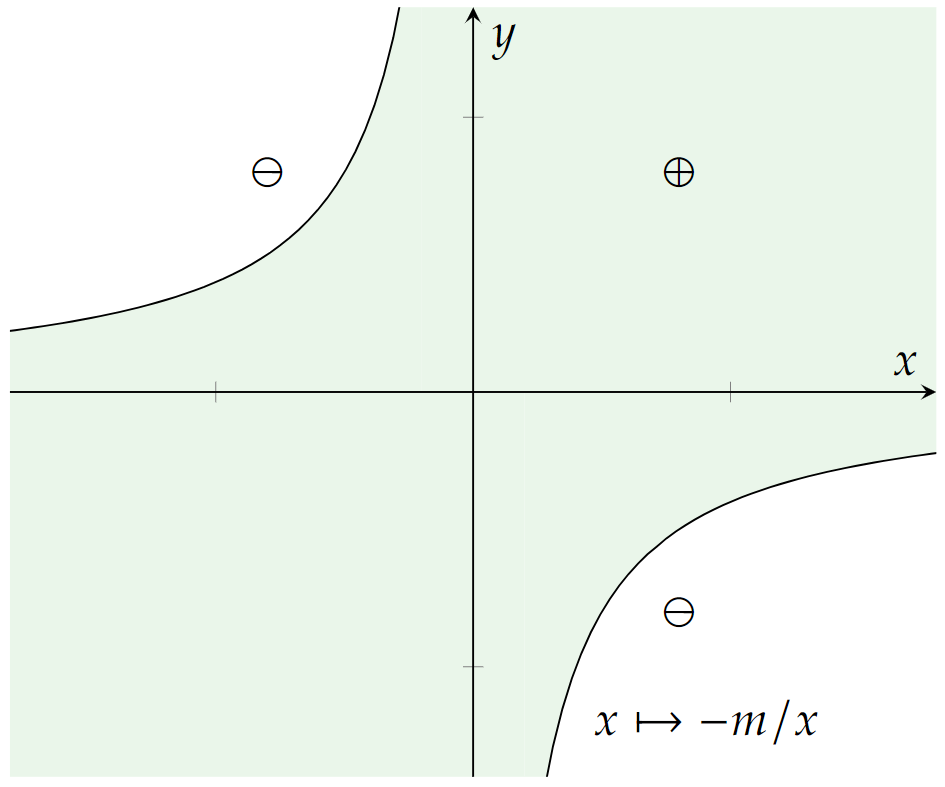
\includegraphics[width=\textwidth]{figures/submod.png}
                \label{fig:submod}
            \end{figure}
        \end{column}
        \begin{column}[t]{.5\textwidth}
            \begin{itemize}
                \item $c(x,y)=-x^2y^2-4mxy$ is submodular on the region $S=\{(x,y)\mid xy\geq -m \}$ if $m\geq0$
                \vspace{1cm}
                \item expect increasing on $S$ and decreasing elsewhere?
            \end{itemize}
        \end{column}
    \end{columns}
\end{frame}


\subsection{Computation of non-monotone optimal plans}
\begin{frame}{Sub-optimality of the monotone rearrangements}
    \begin{block}{Theorem \cite{vayer2020contribution}}
        In the discrete case in dimension 1 with $N=M$ and $a=b=\mathbbm{1}_N$, \emph{either $\pimon$} (eq.~identity $\sigma(i)=i$) \emph{or $\piantimon$} (eq.~anti-identity $\sigma(i)=N+1-i$) \emph{is optimal} for \cref{eqn:GW-quadratic}.
    \end{block}
\begin{itemize}
    \item \textbf{empirically:} very often true when generating points at random
    \item \textbf{literature:} \emph{counter-example} by \cite{beinert2022assignment} for $N\geq 7$ points
    \item \textbf{here:} procedure to \emph{automatically} obtain additional \emph{counter-examples}
\end{itemize}
\pause
\begin{columns}
    \begin{column}[b]{.3\linewidth}
        % This file was created with tikzplotlib v0.10.1.
\begin{tikzpicture}[scale=.65]

    \begin{axis}[
    title={Initial plan $\pi_0$},
    xlabel={$x$},
    ylabel={$y$},
    xmin=-0.860483883693814, xmax=0.860483883693814,
    ymin=-0.98424434363842, ymax=0.98424434363842,
    grid = major,
    axis lines=left,
    axis equal,
    ]
    \addplot [draw=tabpurple, fill=tabpurple, mark=*, only marks,opacity=.6, draw opacity=0]
    table{%
    x  y
    0.555029630661011 -0.0158676505088806
    -0.236768633127213 0.355503797531128
    0.544643044471741 0.104050576686859
    -0.194337338209152 -0.0446888208389282
    -0.283418506383896 -0.407166182994843
    -0.326179891824722 0.230781435966492
    -0.253536850214005 -0.248354732990265
    -0.139955550432205 0.245159804821014
    -0.176041215658188 0.456286549568176
    0.549169182777405 0.334675550460815
    -0.333650857210159 -0.431270480155945
    0.207398444414139 0.353976368904114
    0.156865984201431 -0.382931172847748
    -0.250565379858017 0.308950901031494
    0.261155754327774 -0.470198333263397
    -0.210368067026138 0.0642983317375183
    -0.169332355260849 -0.189902603626251
    0.392874985933304 -0.0384848713874817
    -0.289017468690872 0.260072827339172
    0.382877200841904 -0.194872617721558
    0.322315603494644 0.371125638484955
    0.05231574177742 0.108898401260376
    0.33347424864769 -0.237155020236969
    -0.31975182890892 0.493428528308868
    -0.0101818144321442 -0.30777645111084
    -0.221232026815414 0.152289867401123
    0.147978037595749 0.338643074035645
    -0.317791134119034 -0.303987145423889
    -0.400682240724564 0.395698249340057
    -0.146978765726089 -0.23452764749527
    0.512488603591919 -0.324599802494049
    -0.30556783080101 -0.445916712284088
    -0.0358024537563324 -0.0697241425514221
    -0.0912812650203705 0.187010586261749
    -0.323942273855209 0.0577062368392944
    0.280057102441788 -0.258328318595886
    -0.168274790048599 -0.110755920410156
    0.382387191057205 -0.300583899021149
    -0.29683730006218 -0.345050394535065
    0.149961620569229 -0.124405741691589
    -0.0355304777622223 0.0557541251182556
    -0.0407645404338837 0.284307897090912
    0.0247271358966827 0.27869176864624
    -0.0798503458499908 0.420502126216888
    0.00401011109352112 -0.488527834415436
    -0.413885325193405 -0.397468686103821
    0.395864278078079 0.0138669610023499
    0.0377726256847382 -0.093356728553772
    0.222262471914291 0.398219287395477
    -0.027001291513443 0.0481876134872437
    0.173529058694839 0.45062130689621
    0.095820277929306 0.258765935897827
    -0.185678154230118 0.278037309646606
    0.152429193258286 0.0925498604774475
    0.498135596513748 0.260421872138977
    -0.429192751646042 -0.429079830646515
    -0.0217974483966827 -0.17097008228302
    0.312465757131577 0.383726358413696
    0.0647160112857819 0.311473965644836
    0.247042804956436 0.186284482479095
    -0.275886982679367 0.11732143163681
    -0.0585298240184784 -0.398380994796753
    -0.131526082754135 0.0180906653404236
    -0.382843405008316 0.495713412761688
    0.428420037031174 -0.38513195514679
    0.318877905607224 -0.187862992286682
    -0.0301567018032074 -0.4527707695961
    0.485664933919907 0.403507351875305
    0.373182088136673 0.288419723510742
    -0.198172718286514 -0.407697439193726
    0.0928529798984528 0.129496157169342
    -0.263608783483505 -0.335467755794525
    -0.3370221555233 0.065843939781189
    0.0660794675350189 -0.414897620677948
    -0.204000979661942 0.12734979391098
    0.450773566961288 -0.339365720748901
    0.231547206640244 -0.112659335136414
    0.323924750089645 -0.452231049537659
    0.11105141043663 -0.288233816623688
    -0.207259505987167 -0.088228166103363
    0.0673986375331879 0.209961175918579
    0.383201092481613 -0.45745986700058
    0.259228736162186 -0.397888660430908
    -0.405101984739304 0.356888294219971
    -0.369065493345261 -0.243187546730042
    -0.124457567930222 -0.386952579021454
    -0.102398365736008 0.367921233177185
    -0.30541530251503 0.167475700378418
    -0.425343066453934 0.165306985378265
    0.201642423868179 0.0133430957794189
    -0.0095919668674469 -0.405273020267487
    0.185787290334702 0.493967235088348
    -0.386108547449112 0.228136360645294
    -0.322127968072891 -0.394426882266998
    -0.143171042203903 0.381069421768188
    0.413891106843948 0.289939701557159
    0.225552827119827 0.196329057216644
    -0.245900183916092 0.161448657512665
    0.0844146907329559 0.154719233512878
    -0.179586321115494 0.306278169155121
    0.301403194665909 0.0181658864021301
    -0.177426904439926 -0.306294500827789
    -0.38782075047493 0.394672214984894
    -0.0506928861141205 0.0619080066680908
    0.140196830034256 -0.43829607963562
    0.365351229906082 -0.035691499710083
    0.38993713259697 -0.171832323074341
    0.265565484762192 0.102889955043793
    -0.260365158319473 -0.223024189472198
    -0.323181599378586 0.0323825478553772
    -0.317005842924118 -0.293777823448181
    -0.266747921705246 0.394475519657135
    };
    \end{axis}

    \end{tikzpicture}

        \vspace{-8mm}
    \end{column}
    \begin{column}[b]{.3\linewidth}
        % This file was created with tikzplotlib v0.10.1.
\begin{tikzpicture}[scale=.65]

    \begin{axis}[
    title={Final plan $\pi_f$},
    xlabel={$x$},
    xmin=-0.860483883693814, xmax=0.860483883693814,
    ymin=-0.98424434363842, ymax=0.98424434363842,
    grid = major,
    axis lines=left,
    axis equal,
    ]
    \addplot [draw=tabpurple, fill=tabpurple, mark=*, only marks,opacity=.6, draw opacity=0]
    table{%
    x  y
    -0.0475812740623951 -0.00340059632435441
    -0.0441303513944149 0.0977057367563248
    -0.0442190244793892 0.0718558132648468
    -0.0466805137693882 0.00833576358854771
    -0.0477646812796593 -0.108987741172314
    -0.0413817279040813 0.109386973083019
    -0.0483411774039268 -0.109251156449318
    -0.048307828605175 0.0838327631354332
    -0.0371303409337997 0.0613369047641754
    0.817175030708313 0.897216498851776
    -0.0482831038534641 -0.108428820967674
    -0.0447965525090694 0.110614284873009
    -0.036015722900629 -0.108963027596474
    -0.0438485108315945 0.0945742800831795
    0.0132665485143661 -0.0915598645806313
    -0.0454493500292301 0.0470575354993343
    -0.0483983010053635 -0.0836576446890831
    -0.0449897795915604 -0.00183166423812509
    -0.0481329299509525 0.0934909284114838
    0.00847463868558407 -0.0838896632194519
    -0.0201860945671797 0.110789969563484
    -0.0454405024647713 0.0466846711933613
    0.00794699043035507 -0.10198587924242
    -0.0438002422451973 0.0828163623809814
    -0.0487846024334431 -0.109610706567764
    -0.0438351295888424 0.0812704414129257
    -0.0448389202356339 0.0490087643265724
    -0.047769483178854 -0.109528876841068
    -0.0364673547446728 0.0948797687888145
    -0.0489671863615513 -0.109020784497261
    0.804644048213959 -0.843340396881104
    -0.0490020290017128 -0.109648950397968
    -0.0476549714803696 0.0018444717861712
    -0.0438759811222553 0.0812242925167084
    -0.0450367592275143 0.047038622200489
    -0.00652758218348026 -0.10457718372345
    -0.0476841442286968 -0.0261788815259933
    0.0341730751097202 -0.0964658558368683
    -0.0482552126049995 -0.105813428759575
    -0.0450278036296368 -0.0431392602622509
    -0.0453220792114735 0.0466888211667538
    -0.0454730838537216 0.10557959228754
    -0.0446379743516445 0.0966566875576973
    -0.0439731553196907 0.109578840434551
    -0.0489734932780266 -0.10903537273407
    -0.046284195035696 -0.109579287469387
    -0.0462511293590069 0.0215715114027262
    -0.0470862984657288 -0.0139435715973377
    -0.0438619293272495 0.10637903958559
    -0.0459479764103889 0.0467469207942486
    -0.0447905547916889 0.0636114850640297
    -0.0379205122590065 0.0914457887411118
    -0.0147720724344254 0.110659137368202
    -0.0452795699238777 0.0466407015919685
    0.0134735815227032 0.110991790890694
    -0.0483037307858467 -0.100258551537991
    -0.0478320382535458 -0.0571895390748978
    -0.0187774132937193 0.110866993665695
    -0.0449938513338566 0.0993728265166283
    -0.0436838045716286 0.0743295475840569
    -0.0154984556138515 0.0642513930797577
    -0.0482148230075836 -0.0983421355485916
    -0.046513669192791 0.0302988514304161
    -0.0447973273694515 0.101852312684059
    0.772858798503876 -0.81375914812088
    -0.0150513425469398 -0.0950996652245522
    -0.0488341301679611 -0.109095200896263
    0.558734118938446 0.855513453483582
    -0.0306842885911465 0.102204032242298
    -0.048664890229702 -0.108449772000313
    -0.0476398505270481 0.0466734692454338
    -0.0487281531095505 -0.102116376161575
    -0.0462375953793526 0.0470677465200424
    -0.0489896237850189 -0.109523631632328
    -0.0437434874475002 0.0641783475875854
    0.815857708454132 -0.703193187713623
    -0.0450068674981594 -0.0431612208485603
    0.0342482104897499 -0.110243208706379
    -0.0157681405544281 -0.108991578221321
    -0.0476663447916508 -0.0103251747786999
    -0.0437650494277477 0.0711103230714798
    0.259046137332916 -0.122416362166405
    0.0134525373578072 -0.0671508312225342
    -0.0443049035966396 0.110298775136471
    -0.0489722192287445 -0.109457820653915
    -0.0462229363620281 -0.108776450157166
    -0.0439266040921211 0.103450559079647
    -0.0452461540699005 0.0952032804489136
    -0.0445888079702854 0.109978541731834
    -0.0464168898761272 0.0215739142149687
    -0.0488363690674305 -0.109651520848274
    -0.0439438261091709 0.107009597122669
    -0.0251717530190945 0.102297611534595
    -0.020452544093132 -0.109555952250957
    -0.0438580699265003 0.106445752084255
    -0.0192825943231583 0.110856600105762
    -0.0436716377735138 0.074300192296505
    -0.035883292555809 0.0879584029316902
    -0.0453389137983322 0.0485817119479179
    -0.0447676591575146 0.109777428209782
    -0.0464421845972538 0.0215416569262743
    -0.0471973158419132 -0.109632275998592
    -0.0438513122498989 0.106677636504173
    -0.0439114719629288 0.0467464290559292
    -0.0359955914318562 -0.109192289412022
    -0.0482445061206818 -0.00181822525337338
    0.0022273832000792 -0.107356525957584
    -0.0451836325228214 0.0466696694493294
    -0.0480019599199295 -0.109633311629295
    -0.0447049923241138 0.0470405519008636
    -0.0483166500926018 -0.109632670879364
    -0.0442694015800953 0.0842185094952583
    };
    \end{axis}

    \end{tikzpicture}

        \vspace{-8mm}
    \end{column}
    \begin{column}[b]{.3\linewidth}
        \centering
        % This file was created with tikzplotlib v0.10.1.
\begin{tikzpicture}[scale=.5]

    \begin{axis}[
    title={Objective function $\Ff(\pi)$},
    xlabel={Iterations},
    xmin=-3.25, xmax=68.25,
    ymin=-0.0133060135878623, ymax=0.0390243952162564,
    grid = major,
    axis lines=left,
    ]
    \addplot[ultra thick, no marks, tabblue]
    table {%
    0 0.0366457402706146
    1 0.0128296026960015
    2 0.00764693738892674
    3 0.00516638578847051
    4 0.0037919997703284
    5 0.00292218313552439
    6 0.0023217792622745
    7 0.00190227513667196
    8 0.00157574948389083
    9 0.00134416075889021
    10 0.00114074978046119
    11 0.000998637056909502
    12 0.000866047223098576
    13 0.00076767144491896
    14 0.000676982395816594
    15 0.000603142834734172
    16 0.000542129680979997
    17 0.000482635397929698
    18 0.000441085547208786
    19 0.000394769042031839
    20 0.000358618883183226
    21 0.000328242749674246
    22 0.000294765632133931
    23 0.000271784490905702
    24 0.000246440700720996
    25 0.000222068309085444
    26 0.000205642892979085
    27 0.000186464632861316
    28 0.000164534663781524
    29 0.000155049579916522
    30 0.000136664952151477
    31 0.000118492491310462
    32 0.000111368106445298
    33 9.13372787181288e-05
    34 7.99107947386801e-05
    35 7.14088673703372e-05
    36 5.07369404658675e-05
    37 4.42669843323529e-05
    38 3.13138007186353e-05
    39 1.63891818374395e-05
    40 5.7496945373714e-06
    41 -1.32657296489924e-05
    42 -1.94765452761203e-05
    43 -4.64202603325248e-05
    44 -5.04592899233103e-05
    45 -7.56503432057798e-05
    46 -8.77406564541161e-05
    47 -0.000117279996629804
    48 -0.000136992719490081
    49 -0.000163182790856808
    50 -0.000196536770090461
    51 -0.000234442006330937
    52 -0.000290850817691535
    53 -0.000317854166496545
    54 -0.000384356826543808
    55 -0.00048568716738373
    56 -0.000578868668526411
    57 -0.000735051580704749
    58 -0.000863353256136179
    59 -0.0012065467890352
    60 -0.00146772898733616
    61 -0.00207047536969185
    62 -0.00256216758862138
    63 -0.00445789750665426
    64 -0.00563399493694305
    65 -0.0109273586422205
    };
    \end{axis}

    \end{tikzpicture}

        \vspace{-8mm}
    \end{column}
\end{columns}

\end{frame}
\begin{frame}{Sub-optimality of the monotone rearrangements}
    \begin{columns}
        \begin{column}[b]{.3\linewidth}
            % This file was created with tikzplotlib v0.10.1.
\begin{tikzpicture}[scale=.65]

    \begin{axis}[
    title={Initial plan $\pi_0$},
    xlabel={$x$},
    ylabel={$y$},
    xmin=-0.860483883693814, xmax=0.860483883693814,
    ymin=-0.98424434363842, ymax=0.98424434363842,
    grid = major,
    axis lines=left,
    axis equal,
    ]
    \addplot [draw=tabpurple, fill=tabpurple, mark=*, only marks,opacity=.6, draw opacity=0]
    table{%
    x  y
    0.555029630661011 -0.0158676505088806
    -0.236768633127213 0.355503797531128
    0.544643044471741 0.104050576686859
    -0.194337338209152 -0.0446888208389282
    -0.283418506383896 -0.407166182994843
    -0.326179891824722 0.230781435966492
    -0.253536850214005 -0.248354732990265
    -0.139955550432205 0.245159804821014
    -0.176041215658188 0.456286549568176
    0.549169182777405 0.334675550460815
    -0.333650857210159 -0.431270480155945
    0.207398444414139 0.353976368904114
    0.156865984201431 -0.382931172847748
    -0.250565379858017 0.308950901031494
    0.261155754327774 -0.470198333263397
    -0.210368067026138 0.0642983317375183
    -0.169332355260849 -0.189902603626251
    0.392874985933304 -0.0384848713874817
    -0.289017468690872 0.260072827339172
    0.382877200841904 -0.194872617721558
    0.322315603494644 0.371125638484955
    0.05231574177742 0.108898401260376
    0.33347424864769 -0.237155020236969
    -0.31975182890892 0.493428528308868
    -0.0101818144321442 -0.30777645111084
    -0.221232026815414 0.152289867401123
    0.147978037595749 0.338643074035645
    -0.317791134119034 -0.303987145423889
    -0.400682240724564 0.395698249340057
    -0.146978765726089 -0.23452764749527
    0.512488603591919 -0.324599802494049
    -0.30556783080101 -0.445916712284088
    -0.0358024537563324 -0.0697241425514221
    -0.0912812650203705 0.187010586261749
    -0.323942273855209 0.0577062368392944
    0.280057102441788 -0.258328318595886
    -0.168274790048599 -0.110755920410156
    0.382387191057205 -0.300583899021149
    -0.29683730006218 -0.345050394535065
    0.149961620569229 -0.124405741691589
    -0.0355304777622223 0.0557541251182556
    -0.0407645404338837 0.284307897090912
    0.0247271358966827 0.27869176864624
    -0.0798503458499908 0.420502126216888
    0.00401011109352112 -0.488527834415436
    -0.413885325193405 -0.397468686103821
    0.395864278078079 0.0138669610023499
    0.0377726256847382 -0.093356728553772
    0.222262471914291 0.398219287395477
    -0.027001291513443 0.0481876134872437
    0.173529058694839 0.45062130689621
    0.095820277929306 0.258765935897827
    -0.185678154230118 0.278037309646606
    0.152429193258286 0.0925498604774475
    0.498135596513748 0.260421872138977
    -0.429192751646042 -0.429079830646515
    -0.0217974483966827 -0.17097008228302
    0.312465757131577 0.383726358413696
    0.0647160112857819 0.311473965644836
    0.247042804956436 0.186284482479095
    -0.275886982679367 0.11732143163681
    -0.0585298240184784 -0.398380994796753
    -0.131526082754135 0.0180906653404236
    -0.382843405008316 0.495713412761688
    0.428420037031174 -0.38513195514679
    0.318877905607224 -0.187862992286682
    -0.0301567018032074 -0.4527707695961
    0.485664933919907 0.403507351875305
    0.373182088136673 0.288419723510742
    -0.198172718286514 -0.407697439193726
    0.0928529798984528 0.129496157169342
    -0.263608783483505 -0.335467755794525
    -0.3370221555233 0.065843939781189
    0.0660794675350189 -0.414897620677948
    -0.204000979661942 0.12734979391098
    0.450773566961288 -0.339365720748901
    0.231547206640244 -0.112659335136414
    0.323924750089645 -0.452231049537659
    0.11105141043663 -0.288233816623688
    -0.207259505987167 -0.088228166103363
    0.0673986375331879 0.209961175918579
    0.383201092481613 -0.45745986700058
    0.259228736162186 -0.397888660430908
    -0.405101984739304 0.356888294219971
    -0.369065493345261 -0.243187546730042
    -0.124457567930222 -0.386952579021454
    -0.102398365736008 0.367921233177185
    -0.30541530251503 0.167475700378418
    -0.425343066453934 0.165306985378265
    0.201642423868179 0.0133430957794189
    -0.0095919668674469 -0.405273020267487
    0.185787290334702 0.493967235088348
    -0.386108547449112 0.228136360645294
    -0.322127968072891 -0.394426882266998
    -0.143171042203903 0.381069421768188
    0.413891106843948 0.289939701557159
    0.225552827119827 0.196329057216644
    -0.245900183916092 0.161448657512665
    0.0844146907329559 0.154719233512878
    -0.179586321115494 0.306278169155121
    0.301403194665909 0.0181658864021301
    -0.177426904439926 -0.306294500827789
    -0.38782075047493 0.394672214984894
    -0.0506928861141205 0.0619080066680908
    0.140196830034256 -0.43829607963562
    0.365351229906082 -0.035691499710083
    0.38993713259697 -0.171832323074341
    0.265565484762192 0.102889955043793
    -0.260365158319473 -0.223024189472198
    -0.323181599378586 0.0323825478553772
    -0.317005842924118 -0.293777823448181
    -0.266747921705246 0.394475519657135
    };
    \end{axis}

    \end{tikzpicture}

            \vspace{-8mm}
        \end{column}
        \begin{column}[b]{.3\linewidth}
            % This file was created with tikzplotlib v0.10.1.
\begin{tikzpicture}[scale=.65]

    \begin{axis}[
    title={Final plan $\pi_f$},
    xlabel={$x$},
    xmin=-0.860483883693814, xmax=0.860483883693814,
    ymin=-0.98424434363842, ymax=0.98424434363842,
    grid = major,
    axis lines=left,
    axis equal,
    ]
    \addplot [draw=tabpurple, fill=tabpurple, mark=*, only marks,opacity=.6, draw opacity=0]
    table{%
    x  y
    -0.0475812740623951 -0.00340059632435441
    -0.0441303513944149 0.0977057367563248
    -0.0442190244793892 0.0718558132648468
    -0.0466805137693882 0.00833576358854771
    -0.0477646812796593 -0.108987741172314
    -0.0413817279040813 0.109386973083019
    -0.0483411774039268 -0.109251156449318
    -0.048307828605175 0.0838327631354332
    -0.0371303409337997 0.0613369047641754
    0.817175030708313 0.897216498851776
    -0.0482831038534641 -0.108428820967674
    -0.0447965525090694 0.110614284873009
    -0.036015722900629 -0.108963027596474
    -0.0438485108315945 0.0945742800831795
    0.0132665485143661 -0.0915598645806313
    -0.0454493500292301 0.0470575354993343
    -0.0483983010053635 -0.0836576446890831
    -0.0449897795915604 -0.00183166423812509
    -0.0481329299509525 0.0934909284114838
    0.00847463868558407 -0.0838896632194519
    -0.0201860945671797 0.110789969563484
    -0.0454405024647713 0.0466846711933613
    0.00794699043035507 -0.10198587924242
    -0.0438002422451973 0.0828163623809814
    -0.0487846024334431 -0.109610706567764
    -0.0438351295888424 0.0812704414129257
    -0.0448389202356339 0.0490087643265724
    -0.047769483178854 -0.109528876841068
    -0.0364673547446728 0.0948797687888145
    -0.0489671863615513 -0.109020784497261
    0.804644048213959 -0.843340396881104
    -0.0490020290017128 -0.109648950397968
    -0.0476549714803696 0.0018444717861712
    -0.0438759811222553 0.0812242925167084
    -0.0450367592275143 0.047038622200489
    -0.00652758218348026 -0.10457718372345
    -0.0476841442286968 -0.0261788815259933
    0.0341730751097202 -0.0964658558368683
    -0.0482552126049995 -0.105813428759575
    -0.0450278036296368 -0.0431392602622509
    -0.0453220792114735 0.0466888211667538
    -0.0454730838537216 0.10557959228754
    -0.0446379743516445 0.0966566875576973
    -0.0439731553196907 0.109578840434551
    -0.0489734932780266 -0.10903537273407
    -0.046284195035696 -0.109579287469387
    -0.0462511293590069 0.0215715114027262
    -0.0470862984657288 -0.0139435715973377
    -0.0438619293272495 0.10637903958559
    -0.0459479764103889 0.0467469207942486
    -0.0447905547916889 0.0636114850640297
    -0.0379205122590065 0.0914457887411118
    -0.0147720724344254 0.110659137368202
    -0.0452795699238777 0.0466407015919685
    0.0134735815227032 0.110991790890694
    -0.0483037307858467 -0.100258551537991
    -0.0478320382535458 -0.0571895390748978
    -0.0187774132937193 0.110866993665695
    -0.0449938513338566 0.0993728265166283
    -0.0436838045716286 0.0743295475840569
    -0.0154984556138515 0.0642513930797577
    -0.0482148230075836 -0.0983421355485916
    -0.046513669192791 0.0302988514304161
    -0.0447973273694515 0.101852312684059
    0.772858798503876 -0.81375914812088
    -0.0150513425469398 -0.0950996652245522
    -0.0488341301679611 -0.109095200896263
    0.558734118938446 0.855513453483582
    -0.0306842885911465 0.102204032242298
    -0.048664890229702 -0.108449772000313
    -0.0476398505270481 0.0466734692454338
    -0.0487281531095505 -0.102116376161575
    -0.0462375953793526 0.0470677465200424
    -0.0489896237850189 -0.109523631632328
    -0.0437434874475002 0.0641783475875854
    0.815857708454132 -0.703193187713623
    -0.0450068674981594 -0.0431612208485603
    0.0342482104897499 -0.110243208706379
    -0.0157681405544281 -0.108991578221321
    -0.0476663447916508 -0.0103251747786999
    -0.0437650494277477 0.0711103230714798
    0.259046137332916 -0.122416362166405
    0.0134525373578072 -0.0671508312225342
    -0.0443049035966396 0.110298775136471
    -0.0489722192287445 -0.109457820653915
    -0.0462229363620281 -0.108776450157166
    -0.0439266040921211 0.103450559079647
    -0.0452461540699005 0.0952032804489136
    -0.0445888079702854 0.109978541731834
    -0.0464168898761272 0.0215739142149687
    -0.0488363690674305 -0.109651520848274
    -0.0439438261091709 0.107009597122669
    -0.0251717530190945 0.102297611534595
    -0.020452544093132 -0.109555952250957
    -0.0438580699265003 0.106445752084255
    -0.0192825943231583 0.110856600105762
    -0.0436716377735138 0.074300192296505
    -0.035883292555809 0.0879584029316902
    -0.0453389137983322 0.0485817119479179
    -0.0447676591575146 0.109777428209782
    -0.0464421845972538 0.0215416569262743
    -0.0471973158419132 -0.109632275998592
    -0.0438513122498989 0.106677636504173
    -0.0439114719629288 0.0467464290559292
    -0.0359955914318562 -0.109192289412022
    -0.0482445061206818 -0.00181822525337338
    0.0022273832000792 -0.107356525957584
    -0.0451836325228214 0.0466696694493294
    -0.0480019599199295 -0.109633311629295
    -0.0447049923241138 0.0470405519008636
    -0.0483166500926018 -0.109632670879364
    -0.0442694015800953 0.0842185094952583
    };
    \end{axis}

    \end{tikzpicture}

            \vspace{-8mm}
        \end{column}
        \begin{column}[b]{.3\linewidth}
            \centering
            % This file was created with tikzplotlib v0.10.1.
\begin{tikzpicture}[scale=.5]

    \begin{axis}[
    title={Objective function $\Ff(\pi)$},
    xlabel={Iterations},
    xmin=-3.25, xmax=68.25,
    ymin=-0.0133060135878623, ymax=0.0390243952162564,
    grid = major,
    axis lines=left,
    ]
    \addplot[ultra thick, no marks, tabblue]
    table {%
    0 0.0366457402706146
    1 0.0128296026960015
    2 0.00764693738892674
    3 0.00516638578847051
    4 0.0037919997703284
    5 0.00292218313552439
    6 0.0023217792622745
    7 0.00190227513667196
    8 0.00157574948389083
    9 0.00134416075889021
    10 0.00114074978046119
    11 0.000998637056909502
    12 0.000866047223098576
    13 0.00076767144491896
    14 0.000676982395816594
    15 0.000603142834734172
    16 0.000542129680979997
    17 0.000482635397929698
    18 0.000441085547208786
    19 0.000394769042031839
    20 0.000358618883183226
    21 0.000328242749674246
    22 0.000294765632133931
    23 0.000271784490905702
    24 0.000246440700720996
    25 0.000222068309085444
    26 0.000205642892979085
    27 0.000186464632861316
    28 0.000164534663781524
    29 0.000155049579916522
    30 0.000136664952151477
    31 0.000118492491310462
    32 0.000111368106445298
    33 9.13372787181288e-05
    34 7.99107947386801e-05
    35 7.14088673703372e-05
    36 5.07369404658675e-05
    37 4.42669843323529e-05
    38 3.13138007186353e-05
    39 1.63891818374395e-05
    40 5.7496945373714e-06
    41 -1.32657296489924e-05
    42 -1.94765452761203e-05
    43 -4.64202603325248e-05
    44 -5.04592899233103e-05
    45 -7.56503432057798e-05
    46 -8.77406564541161e-05
    47 -0.000117279996629804
    48 -0.000136992719490081
    49 -0.000163182790856808
    50 -0.000196536770090461
    51 -0.000234442006330937
    52 -0.000290850817691535
    53 -0.000317854166496545
    54 -0.000384356826543808
    55 -0.00048568716738373
    56 -0.000578868668526411
    57 -0.000735051580704749
    58 -0.000863353256136179
    59 -0.0012065467890352
    60 -0.00146772898733616
    61 -0.00207047536969185
    62 -0.00256216758862138
    63 -0.00445789750665426
    64 -0.00563399493694305
    65 -0.0109273586422205
    };
    \end{axis}

    \end{tikzpicture}

            \vspace{-8mm}
        \end{column}
    \end{columns}
    \begin{center}
        {\small\capleft Objective function $\Ff$. \capcenter Initial plan $\pi_0$, generated at random. \capright Final plan $\pi_f$.}
    \end{center}
    \textbf{Procedure:}
    \begin{itemize}
        \item ${\pi=\frac{1}{N}\sum_{i=1}^{N}\delta_{(x_{i},y_{i})}}$
        \item move away from measures of optimal plans $\pimon$ and $\piantimon$ by gradient descent:
        $$\mathcal{F}(\pi)\defeq \underbrace{c_{\gw}(\pi)}_{\substack{\text{performance}\\\text{of }\pi}}-\underbrace{\min \left\{ c_{\gw}(\pimon),\, c_{\gw}(\piantimon)\right\}}_{\substack{\text{performance of the monotone}\\\text{rearrangements of the marginals of }\pi}}$$
        \item results similar to \cite{beinert2022assignment}! \light{\faPencil*}
    \end{itemize}
\end{frame}

\begin{frame}{What happens? + computation of optimal bimaps}
    \begin{itemize}
        \item still, $\pimon$ and $\piantimon$ are very often optimal in practice: \emph{what happens?}
        \item generate measures with $N$ points at random and look at the optimal plan for GW! \textbf{how to find it?}\begin{enumerate}
            \item $\pi\opt$ optimal for GW \item $\implies$ optimal for \emph{linearized} $\GW(m(\pi\opt))$
            \item consider all linearized $\GW(m)$ for $m \in [m_\text{min},m_\text{max}]$ and take all optimal plans $\pi\opt_m$ \light{(easy, linear programs!)}
            \item $\pi\opt$ is the one that performs best on GW
        \end{enumerate}
        \pause
        \onslide<2>{
            \vspace{-8mm}
            \begin{figure}
                \centering
                % This file was created with tikzplotlib v0.10.1.
\begin{tikzpicture}[scale=.55]

\begin{axis}[
    xlabel={$m$},
    xmin=-0.194213820111278, xmax=0.194213820111278,
    ymin=-0.290182883647815, ymax=-0.263666083991494,
    grid = major,
    axis lines=left,
    ]
    \addplot[ultra thick, no marks, tabgreen]
table {%
-0.155742431435461 -0.275380102915412
-0.153651929000085 -0.275380102915317
-0.15156142656471 -0.275380102915663
-0.149470924129335 -0.275380102987755
-0.147380421693959 -0.275380102911988
-0.145289919258584 -0.275380102915687
-0.143199416823209 -0.275380102915632
-0.141108914387834 -0.27538010291483
-0.139018411952458 -0.275380102911644
-0.136927909517083 -0.275380102912229
-0.134837407081708 -0.275380102911161
-0.132746904646332 -0.275380102911209
-0.130656402210957 -0.275380102913941
-0.128565899775582 -0.27538010291118
-0.126475397340206 -0.275380102928466
-0.124384894904831 -0.275380102912072
-0.122294392469456 -0.275380102958045
-0.12020389003408 -0.275380102977565
-0.118113387598705 -0.275380102915782
-0.11602288516333 -0.275380102924645
-0.113932382727954 -0.275380102937224
-0.111841880292579 -0.275380102924637
-0.109751377857204 -0.275380102921386
-0.107660875421828 -0.274984380875121
-0.105570372986453 -0.27307776242602
-0.103479870551078 -0.267583241731402
-0.101389368115703 -0.264871393066782
-0.0992988656803272 -0.269701906821325
-0.0972083632449519 -0.273747309218643
-0.0951178608095766 -0.276763076781454
-0.0930273583742013 -0.278452821547287
-0.0909368559388259 -0.279813236302683
-0.0888463535034506 -0.280699860365686
-0.0867558510680753 -0.28176530988425
-0.0846653486327 -0.282626579964681
-0.0825748461973247 -0.283285925684313
-0.0804843437619494 -0.284162356477211
-0.0783938413265741 -0.284596226405426
-0.0763033388911987 -0.285460495863862
-0.0742128364558234 -0.285695449385922
-0.0721223340204481 -0.285892615172939
-0.0700318315850728 -0.286140632459021
-0.0679413291496975 -0.286291203951305
-0.0658508267143222 -0.286528382400582
-0.0637603242789468 -0.286661385181496
-0.0616698218435715 -0.286874006233074
-0.0595793194081962 -0.287008310556664
-0.0574888169728209 -0.287203025927852
-0.0553983145374456 -0.28731435847981
-0.0533078121020703 -0.287490792079257
-0.051217309666695 -0.287601645619975
-0.0491268072313197 -0.287759349811789
-0.0470363047959443 -0.287847550132569
-0.044945802360569 -0.287987820154035
-0.0428552999251937 -0.288070168457747
-0.0407647974898184 -0.288188981177386
-0.0386742950544431 -0.288253888132255
-0.0365837926190678 -0.288362513098762
-0.0344932901836924 -0.288504547888517
-0.0324027877483171 -0.288552644712416
-0.0303122853129418 -0.2886241279915
-0.0282217828775665 -0.288666286619716
-0.0261312804421912 -0.288726360913962
-0.0240407780068159 -0.288802376062399
-0.0219502755714406 -0.288830628490637
-0.0198597731360652 -0.288868156612365
-0.0177692707006899 -0.288913102027494
-0.0156787682653146 -0.288926480081151
-0.0135882658299393 -0.288954796580086
-0.011497763394564 -0.288966902554207
-0.00940726095918867 -0.288976148368565
-0.00731675852381336 -0.288977574572528
-0.00522625608843805 -0.288976667376545
-0.00313575365306271 -0.288957787719671
-0.00104525121768739 -0.288923093581993
0.00104525121768792 -0.288923093581994
0.00313575365306323 -0.288957787719671
0.00522625608843855 -0.288976667376545
0.00731675852381386 -0.288977574572528
0.00940726095918917 -0.288976148368565
0.0114977633945645 -0.288966902554208
0.0135882658299398 -0.288954796580086
0.0156787682653151 -0.28892648008115
0.0177692707006904 -0.288913102027494
0.0198597731360657 -0.288868156612365
0.0219502755714411 -0.288830628490636
0.0240407780068164 -0.288802376062399
0.0261312804421917 -0.288726360913963
0.028221782877567 -0.288666286619716
0.0303122853129423 -0.2886241279915
0.0324027877483176 -0.288552644712416
0.034493290183693 -0.288504547888517
0.0365837926190683 -0.288362513098762
0.0386742950544436 -0.288253888132256
0.0407647974898189 -0.288188981177385
0.0428552999251942 -0.288070168457747
0.0449458023605695 -0.287987820154035
0.0470363047959448 -0.287847550132569
0.0491268072313202 -0.287759349811789
0.0512173096666955 -0.287601645619975
0.0533078121020708 -0.287490792079257
0.0553983145374461 -0.28731435847981
0.0574888169728214 -0.287203025927852
0.0595793194081967 -0.287008310556665
0.061669821843572 -0.286874006233074
0.0637603242789474 -0.286661385181495
0.0658508267143227 -0.286528382400582
0.067941329149698 -0.286291203951305
0.0700318315850733 -0.286140632459021
0.0721223340204486 -0.285892615172939
0.0742128364558239 -0.285695449385923
0.0763033388911993 -0.285460495863862
0.0783938413265746 -0.284596226405427
0.0804843437619499 -0.284162356477211
0.0825748461973252 -0.283285925684313
0.0846653486327005 -0.282626579964682
0.0867558510680758 -0.28176530988425
0.0888463535034511 -0.280699860365683
0.0909368559388264 -0.279813236302684
0.0930273583742018 -0.278452821547288
0.0951178608095771 -0.276763076781455
0.0972083632449524 -0.273747309218644
0.0992988656803277 -0.269701906821326
0.101389368115703 -0.264871393066782
0.103479870551078 -0.267583241731403
0.105570372986454 -0.273077762426022
0.107660875421829 -0.274984380875123
0.109751377857204 -0.275380102921387
0.11184188029258 -0.275380102924638
0.113932382727955 -0.275380102937226
0.11602288516333 -0.275380102924646
0.118113387598706 -0.275380102915784
0.120203890034081 -0.275380102977567
0.122294392469456 -0.275380102958047
0.124384894904831 -0.275380102912074
0.126475397340207 -0.275380102928468
0.128565899775582 -0.275380102911182
0.130656402210957 -0.275380102913942
0.132746904646333 -0.275380102911211
0.134837407081708 -0.275380102911163
0.136927909517083 -0.27538010291223
0.139018411952459 -0.275380102911646
0.141108914387834 -0.275380102914831
0.143199416823209 -0.275380102915633
0.145289919258585 -0.275380102915689
0.14738042169396 -0.275380102911989
0.149470924129335 -0.275380102987756
0.151561426564711 -0.275380102915665
0.153651929000086 -0.275380102915319
0.155742431435461 -0.275380102915413
};
\addplot [thick, dashed]
table {%
-0.155742431435461 -0.275380102915412
-0.155742431435461 -0.290182883647815
} node[above right] {$m_\text{min}$};
\addplot [thick, dashed]
table {%
0.155742431435461 -0.275380102915413
0.155742431435461 -0.290182883647815
} node[above left] {$m_\text{max}$};
\addplot[ultra thick, tabgreen, only marks, mark=*]
table {%
-0.155742431435461 -0.275380102915412
0.155742431435461 -0.275380102915413
};
\end{axis}
\end{tikzpicture}

                \vspace{-8mm}
                \caption{Graph of $m\mapsto \GW(\pi\opt_m)$.}
            \end{figure}}
    \end{itemize}
\end{frame}
\begin{frame}{What happens? + computation of optimal bimaps}
    \begin{itemize}
        \item \textbf{Note:} sum of Diracs $\mu=(X,\mathbbm{1}_N)$ $\to$ density $\mu=(\hat X,a)$ by convolution with small Gaussian $\sigma$
        \item evolution of $\pi\opt_m$ as a function of $m$
        \begin{itemize}
            \item with $N$ random points: \href{./figures/gif_random_full.gif}{\emph{[all]}}, \href{./figures/gif_random_zoom.gif}{\emph{[zoom]}}
            \pause
            \item with counter-examples of before: \href{./figures/gif_full.gif}{\emph{[all]}}, \href{./figures/gif_zoom.gif}{\emph{[zoom]}}
        \end{itemize}
        \item \textbf{Note:} \textit{a priori} no reason to work, and indeed it does not work most of the time
    \end{itemize}
\end{frame}
\begin{frame}{Computation of optimal bimaps}
            \begin{algorithm}[H]
                \caption{Generating bimaps from adversarial examples.}
                \label{algorithm:bimap}
            \vspace{-2mm}
            \textbf{Input:} an adversarial plan $\pi_f=\id(X_f,Y_f)$\\
            \noindent\textbf{Parameters:} $\sigma$, $N_{\Delta x}$, $N_{\Delta m}$\\
            \textbf{Algorithm:}
            \begin{algorithmic}[1]
                \State $a\gets \texttt{convolution}(X_f,\sigma,N_{\Delta x})$
                \State $b\gets \texttt{convolution}(Y_f,\sigma,N_{\Delta x})$ \Comment{(optional)}
                \State $m_{\text{min}}\gets \min_{\pi\in U(a,b)}\ \langle C_{xy},\,\pi\rangle$ \Comment{solve linear programs}
                \State $m_{\text{max}}\gets \max_{\pi\in U(a,b)}\ \langle C_{xy},\,\pi\rangle$
                \State \light{\texttt{GW\_scores} $\gets \texttt{[]}$}
                \For{$m\in\{m_\text{min},\dots,m_\text{max}\}$} \Comment{with $N_{\Delta m}$ points}
                    \State $\pi\opt_m\gets \argmin_{\pi\in U(a,b)}\ \langle C_{\GW(m)},\,\pi\rangle$ \Comment{solve linear program}
                    \State \light{append $\GW(\pi\opt_m)$ to \texttt{GW\_scores}}
                \EndFor
                \State $\pi\opt\gets\argmax_\pi$ \texttt{GW\_scores} \Comment{take best plan for GW}
                \State return $\pi\opt$
                \end{algorithmic}
            \textbf{Outputs:} $\pi\opt$ optimal for GW
          \end{algorithm}
\end{frame}
\begin{frame}{Computation of optimal bimaps}
    \begin{columns}
        \centering
        \begin{column}[b]{.4\linewidth}
            \centering
            % This file was created with tikzplotlib v0.10.1.
\begin{tikzpicture}[scale=.7]

    \begin{axis}[
    % title={Primal variable $\pi$},
    % xlabel={$x$},
    % ylabel={$y$},
    axis on top,
    axis lines=center,
    every axis x label/.style={at={(current axis.right of origin)},anchor=west},
    every axis y label/.style={at={(current axis.above origin)},anchor=east},
    xmin=-3.8, xmax=149.5,
    ymin=-3.8, ymax=149.5,
    y=1.25,
    x=1.25,
    xtick={0,25,50,75,100,125,150},
    xticklabels={,,$50$,,$100$,,$150$},
    ytick={0,25,50,75,100,125,150},
    yticklabels={,,$50$,,$100$,,$150$},
    every tick label/.append style={font=\footnotesize},
    ]
    \addplot graphics [includegraphics cmd=\pgfimage,xmin=-0.5, xmax=149.5, ymin=-0.5, ymax=149.5] {figures/bimap_plan_double-1};
    % \addplot[opacity=.1] graphics [includegraphics cmd=\pgfimage,xmin=-0.5, xmax=149.5, ymin=-0.5, ymax=149.5] {figures/bimap_plan_double-2};
    \addplot[opacity=.1] graphics [includegraphics cmd=\pgfimage,xmin=-0.5, xmax=149.5, ymin=-0.5, ymax=149.5] {figures/bimap_plan_double-3};
    % \addlegendentry{plan}
\addplot [draw=tabblue!80, fill=tabblue!80, mark=square*, mark size=0.45, only marks]
table{%
x  y
-1 77
-1 78
-1 79
};
\addplot [draw=tabblue!80, fill=tabblue!80, mark=square*, mark size=0.45, only marks]
table{%
x  y
-2 77
-2 78
-2 79
};
    \addplot [draw=tabblue!80, fill=tabblue!80, mark=square*, mark size=0.45, only marks]
    table{%
x  y
1 -1
3 -1
4 -1
5 -1
6 -1
7 -1
8 -1
9 -1
10 -1
11 -1
12 -1
13 -1
14 -1
15 -1
16 -1
17 -1
18 -1
19 -1
20 -1
21 -1
22 -1
23 -1
24 -1
25 -1
26 -1
27 -1
28 -1
29 -1
30 -1
31 -1
32 -1
33 -1
34 -1
35 -1
36 -1
37 -1
38 -1
39 -1
40 -1
41 -1
42 -1
43 -1
44 -1
45 -1
46 -1
47 -1
48 -1
49 -1
50 -1
51 -1
52 -1
53 -1
54 -1
55 -1
56 -1
57 -1
58 -1
59 -1
60 -1
61 -1
62 -1
63 -1
64 -1
65 -1
66 -1
67 -1
68 -1
69 -1
70 -1
71 -1
72 -1
73 -1
74 -1
75 -1
76 -1
77 -1
78 -1
79 -1
80 -1
81 -1
82 -1
137 -1
139 -1
141 -1
142 -1
144 -1
    };
    \addplot [draw=tabblue!80, fill=tabblue!80, mark=square*, mark size=0.45, only marks]
    table{%
x  y
1 -2
3 -2
4 -2
5 -2
6 -2
7 -2
8 -2
9 -2
10 -2
11 -2
12 -2
13 -2
14 -2
15 -2
16 -2
17 -2
18 -2
19 -2
20 -2
21 -2
22 -2
23 -2
24 -2
25 -2
26 -2
27 -2
28 -2
29 -2
30 -2
31 -2
32 -2
33 -2
34 -2
35 -2
36 -2
37 -2
38 -2
39 -2
40 -2
41 -2
42 -2
43 -2
44 -2
45 -2
46 -2
47 -2
48 -2
49 -2
50 -2
51 -2
52 -2
53 -2
54 -2
55 -2
56 -2
57 -2
58 -2
59 -2
60 -2
61 -2
62 -2
63 -2
64 -2
65 -2
66 -2
67 -2
68 -2
69 -2
70 -2
71 -2
72 -2
73 -2
74 -2
75 -2
76 -2
77 -2
78 -2
79 -2
80 -2
81 -2
82 -2
137 -2
139 -2
141 -2
142 -2
144 -2
    };
    % \addlegendentry{bimap}
    % \addlegendentry{anti-bimap}

\end{axis}

    \end{tikzpicture}
            \vspace{-8mm}
        \end{column}
        \hfill
        \begin{column}[b]{.49\linewidth}
            \centering
            % This file was created with tikzplotlib v0.10.1.
\begin{tikzpicture}[scale=1]

    \begin{axis}[
    xlabel={$x$},
    ylabel={$y$},
    axis on top,
    axis lines=center,
    every axis x label/.style={at={(current axis.right of origin)},anchor=west},
    every axis y label/.style={at={(current axis.above origin)},anchor=east},
    xmin=-3.8, xmax=149.5,
    ymin=-3.8, ymax=111.5,
    y=1.25,
    x=1.25,
    xtick={0,25,50,75,100,125,150},
    xticklabels={,,$50$,,$100$,,$150$},
    ytick={0,25,50,75,100},
    yticklabels={,,$50$,,$100$},
    every tick label/.append style={font=\footnotesize},
    ]
    \addplot graphics [includegraphics cmd=\pgfimage,xmin=-0.5, xmax=149.5, ymin=-0.5, ymax=111.5] {figures/bimap_plan_bis-1};
    \addplot[opacity=.1] graphics [includegraphics cmd=\pgfimage,xmin=-0.5, xmax=149.5, ymin=-0.5, ymax=111.5] {figures/bimap_plan_bis-3};
    \addplot [draw=tabblue!80, fill=tabblue!80, mark=square*, mark size=0.45, only marks]
    table{%
    143 -1
    145 -1
    146 -1
    };
    \addplot [draw=tabblue!80, fill=tabblue!80, mark=square*, mark size=0.45, only marks]
    table{%
    x  y
    143 -2
    145 -2
    146 -2
    };

\end{axis}

    \end{tikzpicture}

            \vspace{-8mm}
        \end{column}
    \end{columns}
    \begin{figure}[h]
            \caption{Optimal correspondence plan $\pi\opt$ (in log scale), \capleft starting from a plan with both marginals convolved or \capright with only $\mu$ convolved. Parameters: $\sigma=\smash{5.10^{-3}}$, $N_{\Delta x}=150$, $N_{\Delta m}=2000$.
            }
    \end{figure}
    \vspace{-1cm}
    \begin{itemize}
        \item small bimap region for \capright?
        \item ``but it's a map from $\Yy$ to $\Xx$!'' no, in both cases, no map neither $\mu\to\nu$ nor $\nu\to\mu$
    \end{itemize}
\end{frame}

\subsection{Instability of the optimality of monotone optimal plans}
\begin{frame}{Instability of the optimality of monotone rearrangements}
    \begin{block}{Question}
        Is having $\pimon$ or $\piantimon$ as optimal \emph{stable}?
    \end{block}
    \begin{itemize}
        \item minimum are optimal correspondence plans \only<2>{\begin{itemize}
            \item small $\sigma$: optimal plan not monotone by construction;
            \item large $\sigma$: monotone are optimal again.
            \item \emph{phase transition:} landscape of $m\mapsto \GW(\pi\opt_m)$ while increasing $\sigma$
        \end{itemize}}
    \end{itemize}
    \only<1>{
        \vspace{-7mm}
        \begin{figure}
            \centering
            % This file was created with tikzplotlib v0.10.1.
\begin{tikzpicture}[scale=.55]

\begin{axis}[
    xlabel={$m$},
    xmin=-0.194213820111278, xmax=0.194213820111278,
    ymin=-0.290182883647815, ymax=-0.263666083991494,
    grid = major,
    axis lines=left,
    ]
    \addplot[ultra thick, no marks, tabgreen]
table {%
-0.155742431435461 -0.275380102915412
-0.153651929000085 -0.275380102915317
-0.15156142656471 -0.275380102915663
-0.149470924129335 -0.275380102987755
-0.147380421693959 -0.275380102911988
-0.145289919258584 -0.275380102915687
-0.143199416823209 -0.275380102915632
-0.141108914387834 -0.27538010291483
-0.139018411952458 -0.275380102911644
-0.136927909517083 -0.275380102912229
-0.134837407081708 -0.275380102911161
-0.132746904646332 -0.275380102911209
-0.130656402210957 -0.275380102913941
-0.128565899775582 -0.27538010291118
-0.126475397340206 -0.275380102928466
-0.124384894904831 -0.275380102912072
-0.122294392469456 -0.275380102958045
-0.12020389003408 -0.275380102977565
-0.118113387598705 -0.275380102915782
-0.11602288516333 -0.275380102924645
-0.113932382727954 -0.275380102937224
-0.111841880292579 -0.275380102924637
-0.109751377857204 -0.275380102921386
-0.107660875421828 -0.274984380875121
-0.105570372986453 -0.27307776242602
-0.103479870551078 -0.267583241731402
-0.101389368115703 -0.264871393066782
-0.0992988656803272 -0.269701906821325
-0.0972083632449519 -0.273747309218643
-0.0951178608095766 -0.276763076781454
-0.0930273583742013 -0.278452821547287
-0.0909368559388259 -0.279813236302683
-0.0888463535034506 -0.280699860365686
-0.0867558510680753 -0.28176530988425
-0.0846653486327 -0.282626579964681
-0.0825748461973247 -0.283285925684313
-0.0804843437619494 -0.284162356477211
-0.0783938413265741 -0.284596226405426
-0.0763033388911987 -0.285460495863862
-0.0742128364558234 -0.285695449385922
-0.0721223340204481 -0.285892615172939
-0.0700318315850728 -0.286140632459021
-0.0679413291496975 -0.286291203951305
-0.0658508267143222 -0.286528382400582
-0.0637603242789468 -0.286661385181496
-0.0616698218435715 -0.286874006233074
-0.0595793194081962 -0.287008310556664
-0.0574888169728209 -0.287203025927852
-0.0553983145374456 -0.28731435847981
-0.0533078121020703 -0.287490792079257
-0.051217309666695 -0.287601645619975
-0.0491268072313197 -0.287759349811789
-0.0470363047959443 -0.287847550132569
-0.044945802360569 -0.287987820154035
-0.0428552999251937 -0.288070168457747
-0.0407647974898184 -0.288188981177386
-0.0386742950544431 -0.288253888132255
-0.0365837926190678 -0.288362513098762
-0.0344932901836924 -0.288504547888517
-0.0324027877483171 -0.288552644712416
-0.0303122853129418 -0.2886241279915
-0.0282217828775665 -0.288666286619716
-0.0261312804421912 -0.288726360913962
-0.0240407780068159 -0.288802376062399
-0.0219502755714406 -0.288830628490637
-0.0198597731360652 -0.288868156612365
-0.0177692707006899 -0.288913102027494
-0.0156787682653146 -0.288926480081151
-0.0135882658299393 -0.288954796580086
-0.011497763394564 -0.288966902554207
-0.00940726095918867 -0.288976148368565
-0.00731675852381336 -0.288977574572528
-0.00522625608843805 -0.288976667376545
-0.00313575365306271 -0.288957787719671
-0.00104525121768739 -0.288923093581993
0.00104525121768792 -0.288923093581994
0.00313575365306323 -0.288957787719671
0.00522625608843855 -0.288976667376545
0.00731675852381386 -0.288977574572528
0.00940726095918917 -0.288976148368565
0.0114977633945645 -0.288966902554208
0.0135882658299398 -0.288954796580086
0.0156787682653151 -0.28892648008115
0.0177692707006904 -0.288913102027494
0.0198597731360657 -0.288868156612365
0.0219502755714411 -0.288830628490636
0.0240407780068164 -0.288802376062399
0.0261312804421917 -0.288726360913963
0.028221782877567 -0.288666286619716
0.0303122853129423 -0.2886241279915
0.0324027877483176 -0.288552644712416
0.034493290183693 -0.288504547888517
0.0365837926190683 -0.288362513098762
0.0386742950544436 -0.288253888132256
0.0407647974898189 -0.288188981177385
0.0428552999251942 -0.288070168457747
0.0449458023605695 -0.287987820154035
0.0470363047959448 -0.287847550132569
0.0491268072313202 -0.287759349811789
0.0512173096666955 -0.287601645619975
0.0533078121020708 -0.287490792079257
0.0553983145374461 -0.28731435847981
0.0574888169728214 -0.287203025927852
0.0595793194081967 -0.287008310556665
0.061669821843572 -0.286874006233074
0.0637603242789474 -0.286661385181495
0.0658508267143227 -0.286528382400582
0.067941329149698 -0.286291203951305
0.0700318315850733 -0.286140632459021
0.0721223340204486 -0.285892615172939
0.0742128364558239 -0.285695449385923
0.0763033388911993 -0.285460495863862
0.0783938413265746 -0.284596226405427
0.0804843437619499 -0.284162356477211
0.0825748461973252 -0.283285925684313
0.0846653486327005 -0.282626579964682
0.0867558510680758 -0.28176530988425
0.0888463535034511 -0.280699860365683
0.0909368559388264 -0.279813236302684
0.0930273583742018 -0.278452821547288
0.0951178608095771 -0.276763076781455
0.0972083632449524 -0.273747309218644
0.0992988656803277 -0.269701906821326
0.101389368115703 -0.264871393066782
0.103479870551078 -0.267583241731403
0.105570372986454 -0.273077762426022
0.107660875421829 -0.274984380875123
0.109751377857204 -0.275380102921387
0.11184188029258 -0.275380102924638
0.113932382727955 -0.275380102937226
0.11602288516333 -0.275380102924646
0.118113387598706 -0.275380102915784
0.120203890034081 -0.275380102977567
0.122294392469456 -0.275380102958047
0.124384894904831 -0.275380102912074
0.126475397340207 -0.275380102928468
0.128565899775582 -0.275380102911182
0.130656402210957 -0.275380102913942
0.132746904646333 -0.275380102911211
0.134837407081708 -0.275380102911163
0.136927909517083 -0.27538010291223
0.139018411952459 -0.275380102911646
0.141108914387834 -0.275380102914831
0.143199416823209 -0.275380102915633
0.145289919258585 -0.275380102915689
0.14738042169396 -0.275380102911989
0.149470924129335 -0.275380102987756
0.151561426564711 -0.275380102915665
0.153651929000086 -0.275380102915319
0.155742431435461 -0.275380102915413
};
\addplot [thick, dashed]
table {%
-0.155742431435461 -0.275380102915412
-0.155742431435461 -0.290182883647815
} node[above right] {$m_\text{min}$};
\addplot [thick, dashed]
table {%
0.155742431435461 -0.275380102915413
0.155742431435461 -0.290182883647815
} node[above left] {$m_\text{max}$};
\addplot[ultra thick, tabgreen, only marks, mark=*]
table {%
-0.155742431435461 -0.275380102915412
0.155742431435461 -0.275380102915413
};
\end{axis}
\end{tikzpicture}

            \vspace{-8mm}
            \caption{Graph of $m\mapsto \GW(\pi\opt_m)$.}
        \end{figure}}
    \only<2>{\begin{columns}
        \begin{column}[b]{.24\linewidth}
            \centering
            % This file was created with tikzplotlib v0.10.1.
\begin{tikzpicture}[scale=.45]

\begin{axis}[
    xlabel={$m$},
    xmin=-0.194213820111278, xmax=0.194213820111278,
    ymin=-0.290182883647815, ymax=-0.263666083991494,
    grid = major,
    axis lines=left,
    ]
    \addplot[ultra thick, no marks, tabgreen]
table {%
-0.155742431435461 -0.275380102915412
-0.153651929000085 -0.275380102915317
-0.15156142656471 -0.275380102915663
-0.149470924129335 -0.275380102987755
-0.147380421693959 -0.275380102911988
-0.145289919258584 -0.275380102915687
-0.143199416823209 -0.275380102915632
-0.141108914387834 -0.27538010291483
-0.139018411952458 -0.275380102911644
-0.136927909517083 -0.275380102912229
-0.134837407081708 -0.275380102911161
-0.132746904646332 -0.275380102911209
-0.130656402210957 -0.275380102913941
-0.128565899775582 -0.27538010291118
-0.126475397340206 -0.275380102928466
-0.124384894904831 -0.275380102912072
-0.122294392469456 -0.275380102958045
-0.12020389003408 -0.275380102977565
-0.118113387598705 -0.275380102915782
-0.11602288516333 -0.275380102924645
-0.113932382727954 -0.275380102937224
-0.111841880292579 -0.275380102924637
-0.109751377857204 -0.275380102921386
-0.107660875421828 -0.274984380875121
-0.105570372986453 -0.27307776242602
-0.103479870551078 -0.267583241731402
-0.101389368115703 -0.264871393066782
-0.0992988656803272 -0.269701906821325
-0.0972083632449519 -0.273747309218643
-0.0951178608095766 -0.276763076781454
-0.0930273583742013 -0.278452821547287
-0.0909368559388259 -0.279813236302683
-0.0888463535034506 -0.280699860365686
-0.0867558510680753 -0.28176530988425
-0.0846653486327 -0.282626579964681
-0.0825748461973247 -0.283285925684313
-0.0804843437619494 -0.284162356477211
-0.0783938413265741 -0.284596226405426
-0.0763033388911987 -0.285460495863862
-0.0742128364558234 -0.285695449385922
-0.0721223340204481 -0.285892615172939
-0.0700318315850728 -0.286140632459021
-0.0679413291496975 -0.286291203951305
-0.0658508267143222 -0.286528382400582
-0.0637603242789468 -0.286661385181496
-0.0616698218435715 -0.286874006233074
-0.0595793194081962 -0.287008310556664
-0.0574888169728209 -0.287203025927852
-0.0553983145374456 -0.28731435847981
-0.0533078121020703 -0.287490792079257
-0.051217309666695 -0.287601645619975
-0.0491268072313197 -0.287759349811789
-0.0470363047959443 -0.287847550132569
-0.044945802360569 -0.287987820154035
-0.0428552999251937 -0.288070168457747
-0.0407647974898184 -0.288188981177386
-0.0386742950544431 -0.288253888132255
-0.0365837926190678 -0.288362513098762
-0.0344932901836924 -0.288504547888517
-0.0324027877483171 -0.288552644712416
-0.0303122853129418 -0.2886241279915
-0.0282217828775665 -0.288666286619716
-0.0261312804421912 -0.288726360913962
-0.0240407780068159 -0.288802376062399
-0.0219502755714406 -0.288830628490637
-0.0198597731360652 -0.288868156612365
-0.0177692707006899 -0.288913102027494
-0.0156787682653146 -0.288926480081151
-0.0135882658299393 -0.288954796580086
-0.011497763394564 -0.288966902554207
-0.00940726095918867 -0.288976148368565
-0.00731675852381336 -0.288977574572528
-0.00522625608843805 -0.288976667376545
-0.00313575365306271 -0.288957787719671
-0.00104525121768739 -0.288923093581993
0.00104525121768792 -0.288923093581994
0.00313575365306323 -0.288957787719671
0.00522625608843855 -0.288976667376545
0.00731675852381386 -0.288977574572528
0.00940726095918917 -0.288976148368565
0.0114977633945645 -0.288966902554208
0.0135882658299398 -0.288954796580086
0.0156787682653151 -0.28892648008115
0.0177692707006904 -0.288913102027494
0.0198597731360657 -0.288868156612365
0.0219502755714411 -0.288830628490636
0.0240407780068164 -0.288802376062399
0.0261312804421917 -0.288726360913963
0.028221782877567 -0.288666286619716
0.0303122853129423 -0.2886241279915
0.0324027877483176 -0.288552644712416
0.034493290183693 -0.288504547888517
0.0365837926190683 -0.288362513098762
0.0386742950544436 -0.288253888132256
0.0407647974898189 -0.288188981177385
0.0428552999251942 -0.288070168457747
0.0449458023605695 -0.287987820154035
0.0470363047959448 -0.287847550132569
0.0491268072313202 -0.287759349811789
0.0512173096666955 -0.287601645619975
0.0533078121020708 -0.287490792079257
0.0553983145374461 -0.28731435847981
0.0574888169728214 -0.287203025927852
0.0595793194081967 -0.287008310556665
0.061669821843572 -0.286874006233074
0.0637603242789474 -0.286661385181495
0.0658508267143227 -0.286528382400582
0.067941329149698 -0.286291203951305
0.0700318315850733 -0.286140632459021
0.0721223340204486 -0.285892615172939
0.0742128364558239 -0.285695449385923
0.0763033388911993 -0.285460495863862
0.0783938413265746 -0.284596226405427
0.0804843437619499 -0.284162356477211
0.0825748461973252 -0.283285925684313
0.0846653486327005 -0.282626579964682
0.0867558510680758 -0.28176530988425
0.0888463535034511 -0.280699860365683
0.0909368559388264 -0.279813236302684
0.0930273583742018 -0.278452821547288
0.0951178608095771 -0.276763076781455
0.0972083632449524 -0.273747309218644
0.0992988656803277 -0.269701906821326
0.101389368115703 -0.264871393066782
0.103479870551078 -0.267583241731403
0.105570372986454 -0.273077762426022
0.107660875421829 -0.274984380875123
0.109751377857204 -0.275380102921387
0.11184188029258 -0.275380102924638
0.113932382727955 -0.275380102937226
0.11602288516333 -0.275380102924646
0.118113387598706 -0.275380102915784
0.120203890034081 -0.275380102977567
0.122294392469456 -0.275380102958047
0.124384894904831 -0.275380102912074
0.126475397340207 -0.275380102928468
0.128565899775582 -0.275380102911182
0.130656402210957 -0.275380102913942
0.132746904646333 -0.275380102911211
0.134837407081708 -0.275380102911163
0.136927909517083 -0.27538010291223
0.139018411952459 -0.275380102911646
0.141108914387834 -0.275380102914831
0.143199416823209 -0.275380102915633
0.145289919258585 -0.275380102915689
0.14738042169396 -0.275380102911989
0.149470924129335 -0.275380102987756
0.151561426564711 -0.275380102915665
0.153651929000086 -0.275380102915319
0.155742431435461 -0.275380102915413
};
\addplot [thick, dashed]
table {%
-0.155742431435461 -0.275380102915412
-0.155742431435461 -0.290182883647815
} node[above right] {$m_\text{min}$};
\addplot [thick, dashed]
table {%
0.155742431435461 -0.275380102915413
0.155742431435461 -0.290182883647815
} node[above left] {$m_\text{max}$};
\addplot[ultra thick, tabgreen, only marks, mark=*]
table {%
-0.155742431435461 -0.275380102915412
0.155742431435461 -0.275380102915413
};
\end{axis}
\end{tikzpicture}

            \vspace{-8mm}
            \begin{center}{\scriptsize $\sigma_1=8.10^{-3}$}\end{center}
        \end{column}
        \begin{column}[b]{.24\linewidth}
            \centering
            % This file was created with tikzplotlib v0.10.1.
\begin{tikzpicture}[scale=.35]

\begin{axis}[
    xlabel={$m$},
    xmin=-0.194213820111278, xmax=0.194213820111278,
    ymin=-0.298275232893912, ymax=-0.279511366424687,
    grid = major,
    axis lines=left,
    ]
    \addplot[ultra thick, no marks, tabpurple]
table {%
-0.16323869942782 -0.29420231353058
-0.161047575945567 -0.29420231353281
-0.158856452463314 -0.294202313530255
-0.156665328981062 -0.294202313542228
-0.154474205498809 -0.29420231354487
-0.152283082016557 -0.294202313543036
-0.150091958534304 -0.294202313546145
-0.147900835052051 -0.294202313597041
-0.145709711569799 -0.294202313531916
-0.143518588087546 -0.294202313530501
-0.141327464605293 -0.294202313554674
-0.139136341123041 -0.294202313529766
-0.136945217640788 -0.294202313549925
-0.134754094158536 -0.294202313578277
-0.132562970676283 -0.294202313577799
-0.13037184719403 -0.294202313574221
-0.128180723711778 -0.294202313540318
-0.125989600229525 -0.294202313539246
-0.123798476747272 -0.294202313530204
-0.12160735326502 -0.294202313533479
-0.119416229782767 -0.294202313542627
-0.117225106300515 -0.2942023135335
-0.115033982818262 -0.294202313530682
-0.112842859336009 -0.29420231355232
-0.110651735853757 -0.294202313532388
-0.108460612371504 -0.29420231352961
-0.106269488889252 -0.293662003464201
-0.104078365406999 -0.283835622656074
-0.101887241924746 -0.282329170559471
-0.0996961184424937 -0.280364269446016
-0.0975049949602411 -0.282663909440542
-0.0953138714779885 -0.286618941589105
-0.0931227479957358 -0.287823038417687
-0.0909316245134832 -0.288747284047929
-0.0887405010312306 -0.28940306775179
-0.086549377548978 -0.290045396928863
-0.0843582540667254 -0.290690228706021
-0.0821671305844728 -0.29133998132021
-0.0799760071022201 -0.291660691648057
-0.0777848836199675 -0.292296848159351
-0.0755937601377149 -0.292611398746729
-0.0734026366554623 -0.292928548312571
-0.0712115131732097 -0.293541044594295
-0.0690203896909571 -0.29384092002434
-0.0668292662087044 -0.294140977350911
-0.0646381427264518 -0.294430575669961
-0.0624470192441992 -0.29471422157062
-0.0602558957619466 -0.294992688276769
-0.058064772279694 -0.295263736570535
-0.0558736487974413 -0.295523587445989
-0.0536825253151887 -0.295775806092435
-0.0514914018329361 -0.296028200829168
-0.0493002783506835 -0.296264321705584
-0.0471091548684309 -0.296487481539318
-0.0449180313861783 -0.296535813038205
-0.0427269079039257 -0.29668954933424
-0.040535784421673 -0.296869332477093
-0.0383446609394204 -0.296909103237188
-0.0361535374571678 -0.29702454875784
-0.0339624139749152 -0.297063059685438
-0.0317712904926626 -0.297151951060367
-0.0295801670104099 -0.297248783882658
-0.0273890435281573 -0.297272446193699
-0.0251979200459047 -0.297325150689385
-0.0230067965636521 -0.297339704430846
-0.0208156730813995 -0.297377963155265
-0.0186245495991469 -0.297408687000258
-0.0164334261168942 -0.297413887443075
-0.0142423026346416 -0.297422329872583
-0.012051179152389 -0.29742003337139
-0.0098600556701364 -0.297416842358672
-0.00766893218788378 -0.297390534298154
-0.00547780870563117 -0.297313637251217
-0.00328668522337855 -0.297266341387402
-0.00109556174112593 -0.297192861103505
0.00109556174112671 -0.297192861103506
0.00328668522337933 -0.297266341387402
0.00547780870563194 -0.297313637251217
0.00766893218788456 -0.297390534298153
0.00986005567013717 -0.297416842358671
0.0120511791523898 -0.297420033371391
0.0142423026346424 -0.297422329872583
0.016433426116895 -0.297413887443074
0.0186245495991476 -0.297408687000259
0.0208156730814003 -0.297377963155266
0.0230067965636529 -0.297339704430846
0.0251979200459055 -0.297325150689386
0.0273890435281581 -0.2972724461937
0.0295801670104107 -0.297248783882659
0.0317712904926633 -0.297151951060367
0.033962413974916 -0.297063059685437
0.0361535374571686 -0.29702454875784
0.0383446609394212 -0.296909103237188
0.0405357844216738 -0.296869332477093
0.0427269079039264 -0.296689549334241
0.044918031386179 -0.296535813038206
0.0471091548684316 -0.296487481539318
0.0493002783506843 -0.296264321705586
0.0514914018329369 -0.296028200829168
0.0536825253151895 -0.295775806092436
0.0558736487974421 -0.29552358744599
0.0580647722796948 -0.295263736570536
0.0602558957619474 -0.294992688276769
0.0624470192442 -0.29471422157062
0.0646381427264526 -0.294430575669961
0.0668292662087052 -0.294140977350912
0.0690203896909578 -0.29384092002434
0.0712115131732105 -0.293541044594295
0.0734026366554631 -0.292928548312572
0.0755937601377157 -0.292611398746728
0.0777848836199683 -0.29229684815935
0.0799760071022209 -0.29166069164806
0.0821671305844735 -0.291339981320211
0.0843582540667261 -0.290690228706022
0.0865493775489788 -0.290045396928864
0.0887405010312314 -0.289403067751791
0.090931624513484 -0.288747284047931
0.0931227479957366 -0.28782303841769
0.0953138714779893 -0.286618941589107
0.0975049949602418 -0.282663909440544
0.0996961184424945 -0.280364269446017
0.101887241924747 -0.282329170559473
0.104078365407 -0.283835622656077
0.106269488889252 -0.293662003464205
0.108460612371505 -0.294202313529613
0.110651735853758 -0.29420231353239
0.11284285933601 -0.294202313552323
0.115033982818263 -0.294202313530684
0.117225106300515 -0.294202313533503
0.119416229782768 -0.294202313542629
0.121607353265021 -0.294202313533483
0.123798476747273 -0.294202313530207
0.125989600229526 -0.294202313539249
0.128180723711779 -0.29420231354032
0.130371847194031 -0.294202313574224
0.132562970676284 -0.294202313577802
0.134754094158536 -0.29420231357828
0.136945217640789 -0.294202313549927
0.139136341123042 -0.294202313529769
0.141327464605294 -0.294202313554678
0.143518588087547 -0.294202313530504
0.145709711569799 -0.294202313531918
0.147900835052052 -0.294202313597044
0.150091958534305 -0.294202313546148
0.152283082016557 -0.294202313543038
0.15447420549881 -0.294202313544873
0.156665328981063 -0.29420231354223
0.158856452463315 -0.294202313530257
0.161047575945568 -0.294202313532812
0.16323869942782 -0.294202313530582
};
\addplot [thick, dashed]
table {%
-0.16323869942782 -0.29420231353058
-0.16323869942782 -0.298275232893912
};
\addplot [thick, dashed]
table {%
0.16323869942782 -0.294202313530582
0.16323869942782 -0.298275232893912
};
\addplot[ultra thick, tabpurple, only marks, mark=*]
table {%
-0.16323869942782 -0.29420231353058
0.16323869942782 -0.294202313530582
};
\end{axis}

\end{tikzpicture}

            \vspace{-8mm}
            \begin{center}{\scriptsize $\sigma_2=8.8.10^{-3}$}\end{center}
        \end{column}
        \begin{column}[b]{.24\linewidth}
            \centering
            % This file was created with tikzplotlib v0.10.1.
\begin{tikzpicture}[scale=.35]

\begin{axis}[
    xlabel={$m$},
    xmin=-0.194213820111278, xmax=0.194213820111278,
    ymin=-0.307315740861217, ymax=-0.287759251986567,
    grid = major,
    axis lines=left,
    ]
    \addplot[ultra thick, no marks, tabpurple]
table {%
-0.167274033518982 -0.304517718566687
-0.165028744478459 -0.304517718568742
-0.162783455437935 -0.304517718570363
-0.160538166397412 -0.304517718568679
-0.158292877356889 -0.304517718637609
-0.156047588316366 -0.304517718567961
-0.153802299275842 -0.304517718573297
-0.151557010235319 -0.304517718625788
-0.149311721194796 -0.304517718580195
-0.147066432154273 -0.304517718580947
-0.144821143113749 -0.3045177185773
-0.142575854073226 -0.304517718586349
-0.140330565032703 -0.304517718597216
-0.13808527599218 -0.304517718598273
-0.135839986951656 -0.304517718565065
-0.133594697911133 -0.304517718568947
-0.13134940887061 -0.304517718639642
-0.129104119830087 -0.30451771856813
-0.126858830789564 -0.304517718587666
-0.12461354174904 -0.304517718565426
-0.122368252708517 -0.304517718594188
-0.120122963667994 -0.304517718568907
-0.117877674627471 -0.304517718565332
-0.115632385586947 -0.30451771856642
-0.113387096546424 -0.304517718567446
-0.111141807505901 -0.304517718565243
-0.108896518465378 -0.304517718545104
-0.106651229424854 -0.296954358568909
-0.104405940384331 -0.295086143931261
-0.102160651343808 -0.290640125735379
-0.0999153623032845 -0.288557274208142
-0.0976700732627613 -0.289340746876728
-0.095424784222238 -0.292098838299968
-0.0931794951817148 -0.293285863763
-0.0909342061411915 -0.294109239275629
-0.0886889171006683 -0.294839822874232
-0.0864436280601451 -0.295372997474895
-0.0841983390196218 -0.295905292043517
-0.0819530499790986 -0.296441039473682
-0.0797077609385753 -0.296965635697388
-0.0774624718980521 -0.29722601702299
-0.0752171828575288 -0.297745192259393
-0.0729718938170056 -0.29800311597306
-0.0707266047764823 -0.298306263952383
-0.0684813157359591 -0.298742860686472
-0.0662360266954358 -0.298981938238562
-0.0639907376549126 -0.299210806282578
-0.0617454486143894 -0.299433059286501
-0.0595001595738661 -0.299655688711825
-0.0572548705333429 -0.299863500888779
-0.0550095814928196 -0.300063151232501
-0.0527642924522964 -0.300254465410563
-0.0505190034117731 -0.300439775460125
-0.0482737143712499 -0.300609584333982
-0.0460284253307266 -0.300650778686716
-0.0437831362902034 -0.300757744896106
-0.0415378472496801 -0.300886329007365
-0.0392925582091569 -0.30100221947025
-0.0370472691686336 -0.301111586503159
-0.0348019801281104 -0.30121391027529
-0.0325566910875872 -0.301305175367807
-0.0303114020470639 -0.301384993481121
-0.0280661130065407 -0.301490227132168
-0.0258208239660174 -0.301555586045821
-0.0235755349254942 -0.301569823953897
-0.0213302458849709 -0.301591192122879
-0.0190849568444477 -0.301598322595057
-0.0168396678039244 -0.301603028075171
-0.0145943787634012 -0.30159432680194
-0.0123490897228779 -0.301586095549947
-0.0101038006823547 -0.30154924826321
-0.00785851164183143 -0.301491211580021
-0.0056132226013082 -0.301398189251549
-0.00336793356078494 -0.301304339396397
-0.0011226445202617 -0.301198781007987
0.00112264452026153 -0.301198781007986
0.0033679335607848 -0.301304339396397
0.00561322260130803 -0.30139818925155
0.0078585116418313 -0.301491211580021
0.0101038006823545 -0.30154924826321
0.0123490897228778 -0.301586095549947
0.014594378763401 -0.301594326801939
0.0168396678039243 -0.301603028075171
0.0190849568444475 -0.301598322595057
0.0213302458849708 -0.301591192122879
0.023575534925494 -0.301569823953897
0.0258208239660173 -0.301555586045821
0.0280661130065405 -0.301490227132168
0.0303114020470638 -0.301384993481121
0.032556691087587 -0.301305175367807
0.0348019801281103 -0.30121391027529
0.0370472691686335 -0.301111586503159
0.0392925582091567 -0.301002219470249
0.04153784724968 -0.300886329007365
0.0437831362902032 -0.300757744896106
0.0460284253307265 -0.300650778686716
0.0482737143712497 -0.300609584333981
0.050519003411773 -0.300439775460125
0.0527642924522962 -0.300254465410563
0.0550095814928195 -0.300063151232501
0.0572548705333427 -0.299863500888779
0.059500159573866 -0.299655688711825
0.0617454486143892 -0.299433059286501
0.0639907376549124 -0.299210806282578
0.0662360266954357 -0.298981938238561
0.0684813157359589 -0.298742860686472
0.0707266047764822 -0.298306263952382
0.0729718938170054 -0.298003115973061
0.0752171828575287 -0.297745192259393
0.0774624718980519 -0.29722601702299
0.0797077609385752 -0.296965635697387
0.0819530499790984 -0.296441039473682
0.0841983390196217 -0.295905292043516
0.0864436280601449 -0.295372997474895
0.0886889171006681 -0.294839822874232
0.0909342061411914 -0.294109239275629
0.0931794951817147 -0.293285863763004
0.0954247842222379 -0.292098838299968
0.0976700732627611 -0.289340746876729
0.0999153623032844 -0.288557274208142
0.102160651343808 -0.290640125735379
0.104405940384331 -0.295086143931261
0.106651229424854 -0.296954358568909
0.108896518465377 -0.304517718545103
0.111141807505901 -0.304517718565242
0.113387096546424 -0.304517718567445
0.115632385586947 -0.304517718566419
0.11787767462747 -0.304517718565331
0.120122963667994 -0.304517718568907
0.122368252708517 -0.304517718594187
0.12461354174904 -0.304517718565425
0.126858830789563 -0.304517718587666
0.129104119830087 -0.30451771856813
0.13134940887061 -0.304517718639641
0.133594697911133 -0.304517718568946
0.135839986951656 -0.304517718565065
0.13808527599218 -0.304517718598272
0.140330565032703 -0.304517718597214
0.142575854073226 -0.30451771858635
0.144821143113749 -0.3045177185773
0.147066432154273 -0.304517718580947
0.149311721194796 -0.304517718580195
0.151557010235319 -0.304517718625787
0.153802299275842 -0.304517718573296
0.156047588316366 -0.30451771856796
0.158292877356889 -0.304517718637609
0.160538166397412 -0.304517718568679
0.162783455437935 -0.304517718570363
0.165028744478459 -0.304517718568742
0.167274033518982 -0.304517718566687
};
\addplot [thick, dashed]
table {%
-0.167274033518982 -0.304517718566687
-0.167274033518982 -0.307315740861217
};
\addplot [thick, dashed]
table {%
0.167274033518982 -0.304517718566687
0.167274033518982 -0.307315740861217
};
\addplot[ultra thick, tabpurple, only marks, mark=*]
table {%
-0.167274033518982 -0.304517718566687
0.167274033518982 -0.304517718566687
};
\end{axis}

\end{tikzpicture}

            \vspace{-8mm}
            \begin{center}{\scriptsize $\sigma_3=10^{-2}$}\end{center}
        \end{column}
        \begin{column}[b]{.24\linewidth}
            \centering
            % This file was created with tikzplotlib v0.10.1.
\begin{tikzpicture}[scale=.45]

\begin{axis}[
    xlabel={$m$},
    xmin=-0.194213820111278, xmax=0.194213820111278,
    ymin=-0.335194226489427, ymax=-0.304544811107574,
    grid = major,
    axis lines=left,
    ]
    \addplot[ultra thick, no marks, tabgreen]
table {%
-0.17655801828298 -0.331891980335707
-0.174188111997303 -0.331891980319862
-0.171818205711625 -0.331891980283592
-0.169448299425948 -0.331891980223302
-0.16707839314027 -0.331891980243792
-0.164708486854592 -0.331891980263956
-0.162338580568915 -0.331891980286217
-0.159968674283237 -0.331891980247376
-0.15759876799756 -0.331891980285448
-0.155228861711882 -0.331891980281795
-0.152858955426204 -0.331891980278678
-0.150489049140527 -0.33189198026967
-0.148119142854849 -0.331891980230003
-0.145749236569172 -0.331891980218381
-0.143379330283494 -0.33189198026904
-0.141009423997816 -0.331891980235271
-0.138639517712139 -0.331891980245376
-0.136269611426461 -0.331891980236535
-0.133899705140784 -0.331891980234786
-0.131529798855106 -0.331891980237326
-0.129159892569429 -0.331891980281328
-0.126789986283751 -0.331891980316321
-0.124420079998073 -0.331891980319116
-0.122050173712396 -0.33189198032223
-0.119680267426718 -0.331891980219255
-0.117310361141041 -0.331891980221669
-0.114940454855363 -0.331891980219858
-0.112570548569685 -0.331891980305998
-0.110200642284008 -0.331891980243904
-0.10783073599833 -0.331287847826922
-0.105460829712653 -0.330572527047089
-0.103090923426975 -0.326160446720041
-0.100721017141297 -0.323476623849002
-0.0983511108556199 -0.318617854744208
-0.0959812045699423 -0.314451563818012
-0.0936112982842647 -0.311780522830264
-0.0912413919985871 -0.307290484313763
-0.0888714857129096 -0.30631739164939
-0.086501579427232 -0.305931684452569
-0.0841316731415544 -0.305847057261295
-0.0817617668558768 -0.306225122056043
-0.0793918605701992 -0.306719707898304
-0.0770219542845216 -0.30745833888048
-0.074652047998844 -0.307963295225527
-0.0722821417131664 -0.308345071579
-0.0699122354274888 -0.308689571387006
-0.0675423291418113 -0.308823636646417
-0.0651724228561337 -0.309090908398651
-0.0628025165704561 -0.309307871553507
-0.0604326102847785 -0.309543536678146
-0.0580627039991009 -0.309783972735727
-0.0556927977134233 -0.30990452907952
-0.0533228914277457 -0.310067206398183
-0.0509529851420681 -0.310221809017009
-0.0485830788563905 -0.31032126586718
-0.046213172570713 -0.310412832980105
-0.0438432662850354 -0.310491619071646
-0.0414733599993578 -0.310595864116286
-0.0391034537136802 -0.310664756134108
-0.0367335474280026 -0.310714651604707
-0.034363641142325 -0.310754824592714
-0.0319937348566474 -0.310772806989539
-0.0296238285709698 -0.31078712506486
-0.0272539222852923 -0.310790032166037
-0.0248840159996147 -0.310778157852204
-0.0225141097139371 -0.310761086218631
-0.0201442034282595 -0.310735123517862
-0.0177742971425819 -0.310694345336652
-0.0154043908569043 -0.310627228156053
-0.0130344845712267 -0.310579712144007
-0.0106645782855491 -0.310501633602625
-0.00829467199987158 -0.310311126112664
-0.00592476571419398 -0.310172326882364
-0.00355485942851638 -0.310074688943368
-0.00118495314283881 -0.309914842104535
0.00118495314283878 -0.309914842104535
0.00355485942851638 -0.310074688943368
0.00592476571419395 -0.310172326882363
0.00829467199987155 -0.310311126112665
0.0106645782855491 -0.310501633602625
0.0130344845712267 -0.310579712144006
0.0154043908569043 -0.310627228156053
0.0177742971425819 -0.310694345336651
0.0201442034282595 -0.310735123517862
0.0225141097139371 -0.310761086218631
0.0248840159996147 -0.310778157852205
0.0272539222852922 -0.310790032166037
0.0296238285709698 -0.31078712506486
0.0319937348566474 -0.310772806989539
0.034363641142325 -0.310754824592714
0.0367335474280026 -0.310714651604707
0.0391034537136802 -0.310664756134108
0.0414733599993578 -0.310595864116285
0.0438432662850354 -0.310491619071646
0.0462131725707129 -0.310412832980105
0.0485830788563905 -0.31032126586718
0.0509529851420681 -0.310221809017009
0.0533228914277457 -0.310067206398182
0.0556927977134233 -0.309904529079519
0.0580627039991009 -0.309783972735727
0.0604326102847785 -0.309543536678146
0.0628025165704561 -0.309307871553507
0.0651724228561336 -0.309090908398651
0.0675423291418112 -0.308823636646417
0.0699122354274888 -0.308689571387006
0.0722821417131664 -0.308345071579
0.074652047998844 -0.307963295225526
0.0770219542845216 -0.307458338880479
0.0793918605701992 -0.306719707898304
0.0817617668558768 -0.306225122056043
0.0841316731415543 -0.305847057261295
0.086501579427232 -0.305931684452569
0.0888714857129095 -0.306317391649391
0.0912413919985871 -0.307290484313762
0.0936112982842647 -0.311780522830264
0.0959812045699423 -0.314451563818012
0.0983511108556199 -0.318617854744208
0.100721017141297 -0.323476623849002
0.103090923426975 -0.326160446720041
0.105460829712653 -0.330572527047089
0.10783073599833 -0.331287847826922
0.110200642284008 -0.331891980243903
0.112570548569685 -0.331891980305998
0.114940454855363 -0.331891980219857
0.117310361141041 -0.33189198022167
0.119680267426718 -0.331891980219255
0.122050173712396 -0.331891980322229
0.124420079998073 -0.331891980319116
0.126789986283751 -0.331891980316321
0.129159892569429 -0.331891980281327
0.131529798855106 -0.331891980237326
0.133899705140784 -0.331891980234787
0.136269611426461 -0.331891980236535
0.138639517712139 -0.331891980245377
0.141009423997816 -0.331891980235271
0.143379330283494 -0.331891980269039
0.145749236569172 -0.33189198021838
0.148119142854849 -0.331891980230003
0.150489049140527 -0.33189198026967
0.152858955426204 -0.331891980278678
0.155228861711882 -0.331891980281795
0.15759876799756 -0.331891980285447
0.159968674283237 -0.331891980247376
0.162338580568915 -0.331891980286216
0.164708486854592 -0.331891980263955
0.16707839314027 -0.331891980243793
0.169448299425948 -0.331891980223302
0.171818205711625 -0.331891980283591
0.174188111997303 -0.331891980319861
0.17655801828298 -0.331891980335706
};
\addplot [thick, dashed]
table {%
-0.17655801828298 -0.331891980335707
-0.17655801828298 -0.335194226489427
};
\addplot [thick, dashed]
table {%
0.17655801828298 -0.331891980335706
0.17655801828298 -0.335194226489427
};
\addplot[ultra thick, tabgreen, only marks, mark=*]
table {%
-0.17655801828298 -0.331891980335707
0.17655801828298 -0.331891980335706
};
\end{axis}

\end{tikzpicture}

            \vspace{-8mm}
            \begin{center}{\scriptsize $\sigma_4=3.10^{-2}$}\end{center}
        \end{column}
    \end{columns}
    \begin{figure}[h]
        \caption{Graphs of $m\mapsto \GW(\pi\opt_m)$ with \cite{beinert2022assignment}, $N=7$ points.}
    \end{figure}}
\end{frame}

\addtocontents{toc}{\protect\setcounter{tocdepth}{-1}}

\subsection{(A positive result for measures with two components)}
    \begin{frame}{(A positive result for measures with two components)}
        Let $\mu_1$, $\mu_2$, $\nu_1$, $\nu_2$ probability measures on $A \subset \RR$ compact. Fix $t \in (0,1)$ and $K > \operatorname{diam}(A)$. Let $\tau_K : x \mapsto x + K$. Introduce measures
    \begin{equation*}
    \mu = (1-t) \mu_1 + t \tau_{K\pushonly} \mu_2 \quad \text{and}  \quad \nu = (1-t) \nu_1 + t \tau_{K\pushonly} \nu_2\,.
    \end{equation*}

    \begin{figure}[h]
        \centering
        
\begin{tikzpicture}[line cap=round,line join=round,scale=.6]
    \def\margin{.5}
    \def\K{7}
    \def\diam{4}
    \def\height{1.5}
    \def\vertical{2.5}
    \def\spacearrow{.45}
    \def\borellength{.75}
    \def\shade{15}
    % mu
    \draw[tabred,fill=tabred!\shade]
        (0,0)..controls +(70:\diam*0.1) and +(180:\diam*0.1)..
        (\diam/5,0.5*\height)..controls +(0:\diam*0.1) and +(180:\diam*0.1)..
        (2*\diam/5,0.5*\height)..controls +(0:\diam*0.1) and +(180:\diam*0.2)..
        (3*\diam/4,1*\height)..controls +(0:\diam*0.2) and +(110:\diam*0.1)..
        (\diam,0);
    \draw[tabred,fill=tabred!\shade,xshift=\K cm]
        (0,0)..controls +(70:\diam*0.1) and +(180:\diam*0.3)..
        % (\diam/4,2/3*\height)..controls +(0:\diam*0.1) and +(180:\diam*0.1)..
        (\diam/3,.75*\height)..controls +(0:\diam*0.3) and +(140:\diam*0.3)..
        % (3*\diam/4,1*\height)..controls +(0:\diam*0.1) and +(110:\diam*0.1)..
        (\diam,0);
    \draw node[tabred,above] at (-\margin,0) {$\mu$};
    \draw node[tabred,above right] at (.2,0) {$\mu_1$};
    \draw node[tabred,above right] at (.2+\K,0) {$\tau_{K\pushonly}\mu_2$};
    % nu
    \draw[tabblue,fill=tabblue!\shade,yshift=-\vertical cm]
        (0,0)..controls +(70:\diam*0.1) and +(180:\diam*0.1)..
        (\diam/4,1*\height)..controls +(0:\diam*0.1) and +(180:\diam*0.1)..
        (\diam/2,0.5*\height)..controls +(0:\diam*0.1) and +(180:\diam*0.1)..
        (3*\diam/4,2/3*\height)..controls +(0:\diam*0.1) and +(110:\diam*0.1)..
        (\diam,0);
    \draw[tabblue,fill=tabblue!\shade,xshift=\K cm,yshift=-\vertical cm]
        (0,0)..controls +(70:\diam*0.1) and +(180:\diam*0.1)..
        (\diam/4,4/5*\height)..controls +(0:\diam*0.1) and +(180:\diam*0.1)..
        (\diam/2,0.4*\height)..controls +(0:\diam*0.1) and +(180:\diam*0.1)..
        (3*\diam/4,4/5*\height)..controls +(0:\diam*0.1) and +(110:\diam*0.1)..
        (\diam,0);
    \draw node[tabblue,above] at (-\margin,-\vertical) {$\nu_{\vphantom{1}}$};
    \draw node[tabblue,above right] at (.2,-\vertical) {$\nu_1$};
    \draw node[tabblue,above right] at (.2+\K,-\vertical) {$\tau_{K\pushonly}\nu_2$};
    % axis
    \draw[->] (0-\margin,0) -- (\K+\diam+\margin,0);
    \draw node[above right] at (\K +\diam+\margin,0) {$\mathcal{X}$};
    \draw[->,yshift=-\vertical cm] (0-\margin,0) -- (\K +\diam+\margin,0);
    \draw node[above right] at (\K +\diam+\margin,-\vertical) {$\mathcal{Y}$};
    % constants
    \draw[<->,opacity=1,dashed] (0,-\vertical-\spacearrow) -- (\diam,-\vertical-\spacearrow) node[midway,below] {$\operatorname{diam}(A)$};
    % \draw[<->,opacity=1,dashed] (0,-\height-\vertical-\spacearrow) -- (\diam,-\height-\vertical-\spacearrow) node[midway,below] {$\Delta=\operatorname{diam}(A)$};
    % \draw[<->,opacity=1,dashed] (\diam/2,-\height-\vertical+0.1) -- (\K+\diam/2,-\height-\vertical+0.1) node[midway,below] {$K$};
    \draw[<->,opacity=1,dashed] (\diam/2,-\vertical-3*\spacearrow) -- (\K+\diam/2,-\vertical-3*\spacearrow) node[midway,below] {$K$};
    % borel sets
    % \draw[line width=2pt,tabred] (1.25,0) -- (1.25+\borellength,0) node[midway,below] (X) {$X$};
    % \draw[line width=2pt,tabred] (2.75,0) -- (2.75+\borellength,0) node[midway,below] (X') {$X'$};
    % \draw[line width=2pt,tabred] (1.75+\K,0) -- (1.75+\borellength+\K,0) node[midway,below] (X'') {$X''$};
    % \draw[line width=2pt,tabblue] (1.25,-\vertical) -- (1.25+\borellength,-\vertical) node[midway,above] (Y) {$Y$};
    % \draw[line width=2pt,tabblue] (2.75,-\vertical) -- (2.75+\borellength,-\vertical) node[midway,above] (Y') {$Y'$};
    % \draw[line width=2pt,tabblue] (1.75+\K,-\vertical) -- (1.75+\borellength+\K,-\vertical) node[midway,above] (Y'') {$Y''$};
    % \draw[->] (X) -- (Y);
    % \draw[->] (X') -- (Y'') node[near start,left] {$\pi_1\ $};
    % \draw[->] (X'') -- (Y') node[near start,right] {$\ \pi_2$};
    % \draw[->,dashed] (X') -- (Y') node[midway,left] {$\tilde\pi_1$};
    % \draw[->,dashed] (X'') -- (Y'') node[midway,left] {$\tilde\pi_2$};
\end{tikzpicture}



    \end{figure}

    \begin{block}{Theorem}
        For \emph{$K$ large enough}, the unique optimal plan for the quadratic cost between  $\mu$ and $\nu$ is given by \emph{one of the two monotone maps} (increasing or decreasing).
    \end{block}


\end{frame}


\section{Summary \& discussion}
\begin{frame}{Summary \& discussion}
    \textbf{Contributions}
    \begin{enumerate}
        \item \textbf{Thm:} always a \emph{map} for \cref{eqn:GW-inner-prod}
        \item \textbf{Thm:} a \emph{map} or \emph{bimap} for \cref{eqn:GW-quadratic}
        \item \textbf{Conj:} this second claim is \emph{tight}
        \item \textbf{Algo:} \emph{non-optimality} of monotone + \emph{instability} for \cref{eqn:GW-quadratic}
        \item (\textbf{Thm:} monotone rearrangement optimal for \cref{eqn:GW-quadratic} between measures composed of \emph{two distant parts})
    \end{enumerate}
\vfill
\textbf{Very soon:}
\begin{itemize}
    \item remove assumption of compact support
    \item try to show decomposition $\pimon+\piantimon$ for \cref{eqn:GW-quadratic}
\end{itemize}
\vfill
\textbf{Future work:}
\begin{itemize}
    \item quadratic cost: \begin{itemize}
        \item better understanding of the 1d case (maybe simpler)
    \end{itemize}
    \item inner product cost: \begin{itemize}
        \item is \cref{eqn:GW-inner-prod} computationally tractable?
    \end{itemize}
    \item other cost functions \begin{itemize}
        \item apply key lemma to other costs $c_\Xx$ and $c_\Yy$?
    \end{itemize}
\end{itemize}
\end{frame}
\begin{frame}{Links}
    \begin{itemize}
        \item \emph{preprint} on HAL and arxiv: ``\textit{On the existence of Monge maps for the Gromov--Wasserstein distance}'' \light{\href{https://hal.archives-ouvertes.fr/hal-03818500}{https://hal.archives-ouvertes.fr/hal-03818500}}
        \item (soon) \emph{code} on GitHub at \light{\href{https://github.com/theodumont/monge-gromov-wasserstein}{https://github.com/theodumont/monge-gromov-wasserstein}}
    \end{itemize}
\end{frame}
\begin{frame}[standout]
    Thank you!
\end{frame}

\appendix


\begin{frame}[allowframebreaks]{References}

    \bibliography{biblio}
    \bibliographystyle{apalike}

  \end{frame}

\begin{frame}{Inspiration for figures}
    \begin{itemize}
        \item the figure on slides~\ref{slide:fig-transport-1} and~\ref{slide:fig-transport-2}, as well as the ones on slide~\ref{slide:fig-plans} are adapted from \href{https://lchizat.github.io/files/presentations/chizat2019IFCAM_OT.pdf}{\underline{a talk by Lénaïc Chizat}};
        \item the GW figure on slide~\ref{slide:gw} is adapted from \cite{peyre2019computational};
        \item all other figures are my own.
    \end{itemize}
\end{frame}

\end{document}
